\chapter{Kirigami configuration exploration}\label{chap:dataset_study}


Based on the findings in the Pilot Study \cref{chap:pilot_study} we will further explore the effects of Kirigami designs for stretch-depending friction. We are especially interested in the optimization toward friction force and friction coefficient extrema. First, we create a dataset through \acrshort{MD} simulations for an extended set of Kirigami designs. This provides useful insight regarding general trends for the frictonal behavior. Following, we use the dataset to investigate the possibility to use machine learning for a prediction of the friction behavior based on Kirigami design, stretch and load. Finally, we attempt an accelerated search using the acquired machine learning model.


\section{Generating the dataset}
We aim to create a dataset that contains information on frictional behavior for
varying Kirigami configurations \hl{(is it bad to change from ``design'' to
``configuration''...)}, stretch and load. For each configuration, we sample 15
pseudo uniform stretch values (see \cref{sec:stretch_dependency}) between zero
and the rupture stretch according to the rupture test. The normal force is
uniformly sampled in the range $[0.1, 10]$ nN. In total, this gives $3\times 15$
data points for each configuration. For the remaining parameters, we use the
values presented in the pilot study (see \cref{tab:param}). We are mainly
concerned with the mean friction and whether the sheet is ruptured or not.
However, we also include the maximum friction, the relative contact, the rupture
stretch (from the rupture test) and the porosity (void fraction) in the dataset. We generate 68
configurations of the Tetrahedron pattern type, 45 of the Honeycomb type and 100
of the Random walk type. A summary of the dataset is given in
\cref{tab:dataset_summary} while all configurations are shown explicitly in
\cref{sec:dataset_conf}. The Tetrahedron and Honeycomb parameters are chosen to
provide additional variations of the evaluated configurations evaluated in
\cref{chap:pilot_study} which exhibited interesting properties, while the Random
walk configurations are chosen to get as diverse configurations as possible.
Notice that not all submitted data points ``make it'' to the final dataset. This
is due to a small bug in the data generation procedure\footnote{The issue arises from the fact that the rupture point in the rupture test does not
completely match the rupture point in the following simulations. After
performing the rupture test the simulation is restarted with a new substrate
size, corresponding to the measured rupture stretch limit, but also with a new
random velocity and thermostat initialization. The sheet is then stretched and
checkpoints of the simulation state (LAMMPS restart files) are saved for each of
the targeted stretch samples. However, if the rupture point arrives earlier than suggested by the rupture test due, to the randomness from the initialization, some of the planned stretch samples might get lost without a corresponding checkpoint file. Thus, these data points are not included in the dataset even though they ideally should have been noted as a rupture event. This could quite easily have been mitigated by a rewrite of the code, but it was first discovered after the dataset had been created. We notice, however, that the dataset still contains 11.57 \% rupture events which provide a reasonable amount of rupture events to incorporate in the machine learning model}.


\begin{table}[H]
  \begin{center}
  \caption{Summary of the number of generated data points in the dataset. Due to slight deviations in the rupture stretch and the specific numerical procedure not all submitted simulations ``make it'' to the final dataset. Notice that the Tetrahedon (7, 5, 2) and Honeycomb (2, 2, 1, 5) from the pilot study are rerun as a part of the Tetrahedon and the Honeycomb datasets separately. In the latter datasets, the reference point for the pattern is randomized and thus these configurations are not fully identical. This is the reason for the ambiguousness in the total sum.}
  \label{tab:dataset_summary}
  \begin{tabular}{ | c | c | c | c | c |} \hline
  \textbf{Type} & \textbf{Configurations} & \textbf{Submitted data points} & \textbf{Final data points} & \textbf{Ruptures} \\ \hline
  Pilot study & 3 & 270 & 261 & \: 25 \: (9.58 \%)\\ \hline
  Tetrahedon & 68 & 3060 & 3015 & 391 (12.97 \%)\\ \hline
  Honeycomb & 45 & 2025 & 1983 & \: 80 \: (4.03 \%)\\ \hline
  Random walk & 100 & 4500 & 4401 & 622 (14.13 \%) \\ \Xhline{2\arrayrulewidth}
  Total & 214 (216) & 9855 & 9660 & 1118 (11.57 \%) \\ \hline
  \end{tabular}
  \end{center}
\end{table}


\section{Data analysis}
In order to gain insight into the correlations in the data we calculate the correlation coefficients between all variable combinations. More specifically, we calculate the Pearson product-moment correlation coefficient which is defined, between data set $X$ and $Y$, as
\begin{align*}
  \mathrm{corr}(X,Y) = \frac{\mathrm{Cov}(X,Y)}{\sigma_X \sigma_Y} = \frac{\langle (X - \mu_X)(Y - \mu_Y)\rangle}{\sigma_X \sigma_Y} \ \in [-1, 1]
\end{align*}
where $\mathrm{Cov}(X,Y)$ is the covariance, $\mu$ the mean value and $\sigma$ the standard deviation. The correlation coefficients range from a complete negative correlation $(-1)$ through no correlation $(0)$ to a complete positive correlation $(1)$. The correlation coefficients is shown in \cref{fig:corrcoef_matrix}
\begin{figure}[H]
  \centering
  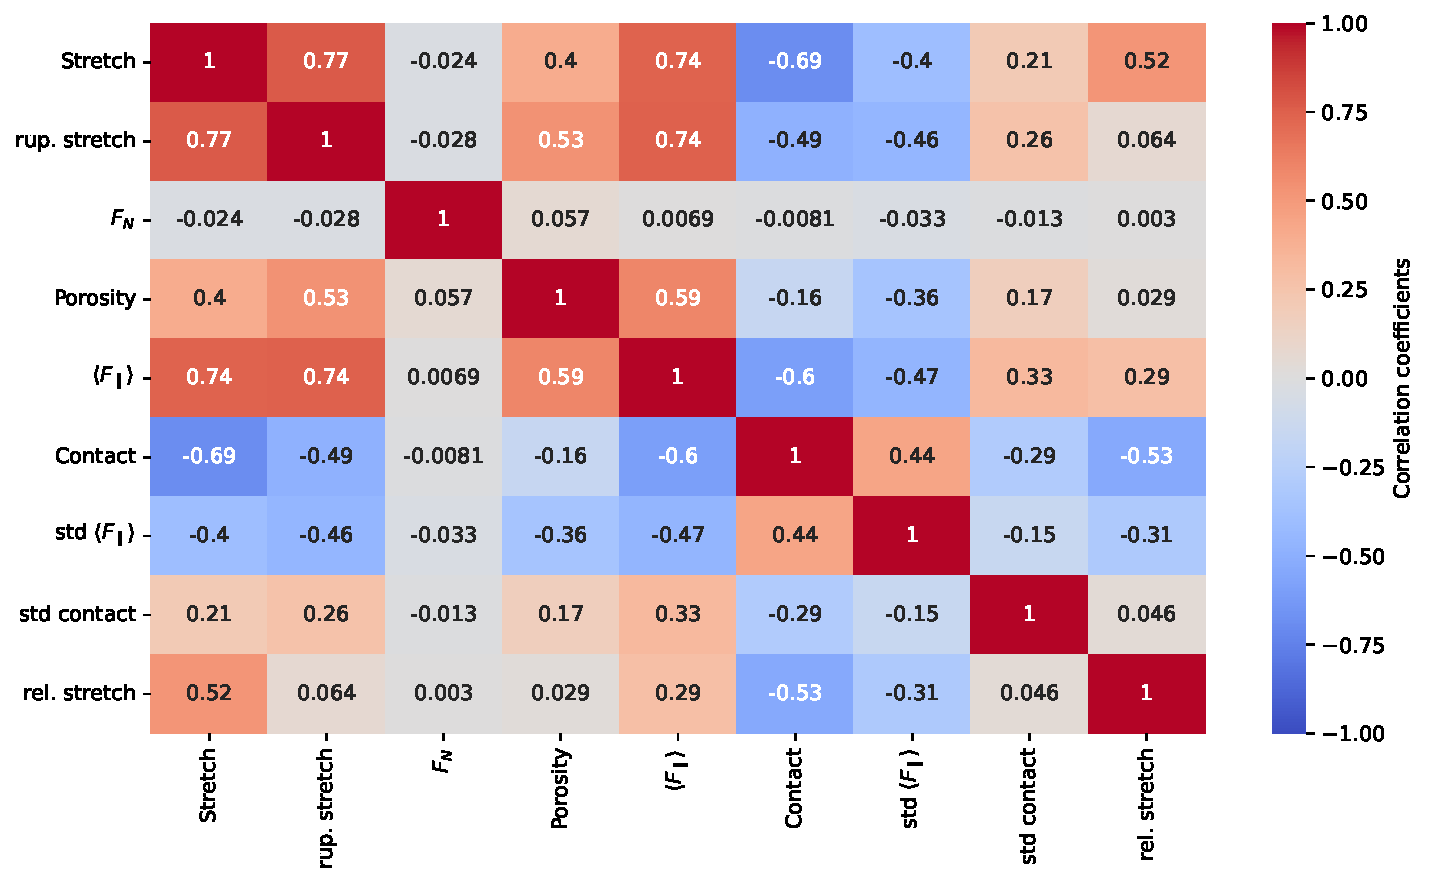
\includegraphics[width=\linewidth]{figures/ML/corrcoef_matrix.pdf}
  \caption{Pearson product-moment correlation coefficients for the full datset (see \cref{tab:dataset_summary}).}
  \label{fig:corrcoef_matrix}
\end{figure}
From \cref{fig:corrcoef_matrix} we especially notice that the mean friction
force $\langle F_{\parallel} \rangle$ has a significant positive correlation
with stretch $(0.77)$ and porosity $(0.60)$. However, the relative stretch, the
stretch scaled by the rupture stretch, has a weaker correlation of only 0.25.
This indicates that the correlation might be associated with the flexibility of
the configurations as these can be taken to higher absolute values of stretch.
This is further supported by the fact that the mean friction and the rupture
stretch are also strongly positively correlated $(0.78)$. From figure
\cref{fig:corrcoef_matrix} we also observe that the contact is negatively
correlated with the mean friction $(-0.67)$ and the stretch value $(-0.74)$
which is consistent with the trend observed in the pilot study in
\cref{fig:multi_stretch} of the contact decreasing with increasing stretch and
mean friction. However, we must take note that the correlation coefficient is a
measure of the strength and slope of a forced linear fit on the data \hl{Do I
need as source?}. Since we have observed a non-linear trend between friction and
stretch (\cref{fig:multi_stretch_mean_fric}) we should not expect any 100 \%
correlations \cref{fig:corr_vis} shown a visualization of the data (excluding
the pilot study configurations) for chosen variable pairs on the axes. This
provides a visual clue on some of the correlations and provides a qualitative
feeling for the diversity in various slices of parameter space that we
eventually are going to base our machine learning model on. We notice that the
honeycomb pattern is spanning a significantly larger range of stretch, contact
and mean friction.

\begin{figure}[H]
  \centering
  \begin{subfigure}[t]{0.49\textwidth}
      \centering
      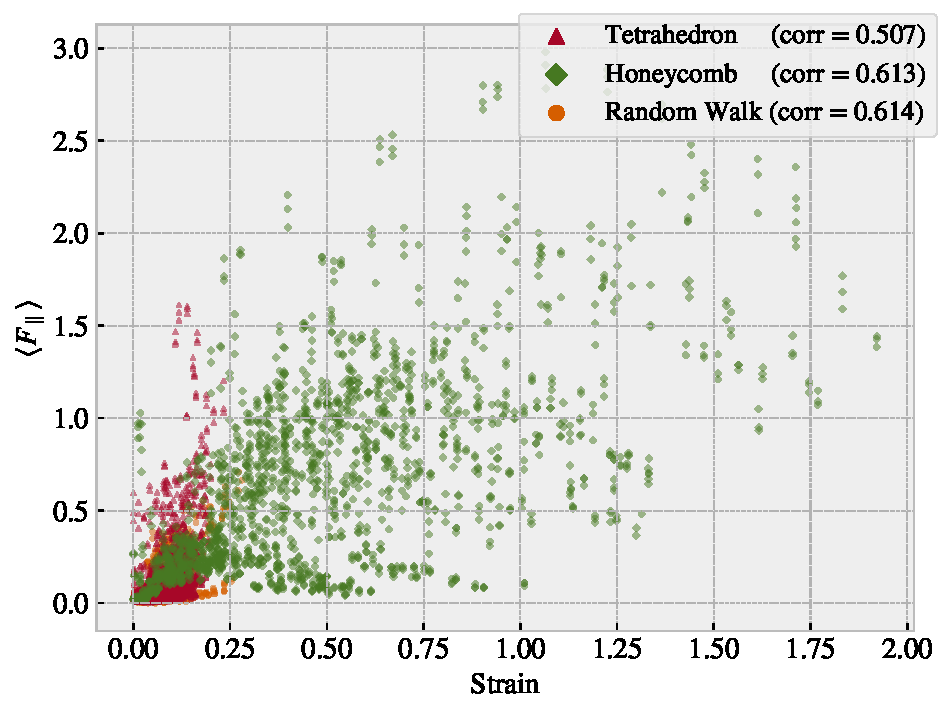
\includegraphics[width=\textwidth]{figures/ML/corr_stretch_Ff.pdf}
      \caption{}
      % \label{fig:}
  \end{subfigure}
  \hfill
  \begin{subfigure}[t]{0.49\textwidth}
      \centering
      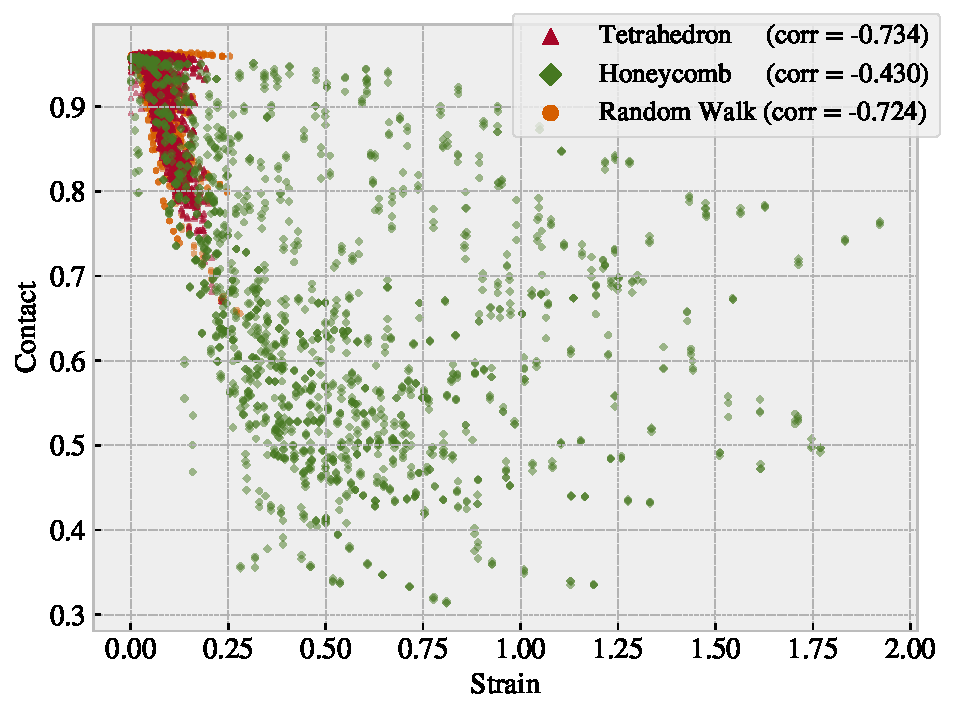
\includegraphics[width=\textwidth]{figures/ML/corr_stretch_contact.pdf}
      \caption{}
      % \label{fig:}
  \end{subfigure}
  \hfill
  \begin{subfigure}[t]{0.49\textwidth}
      \centering
      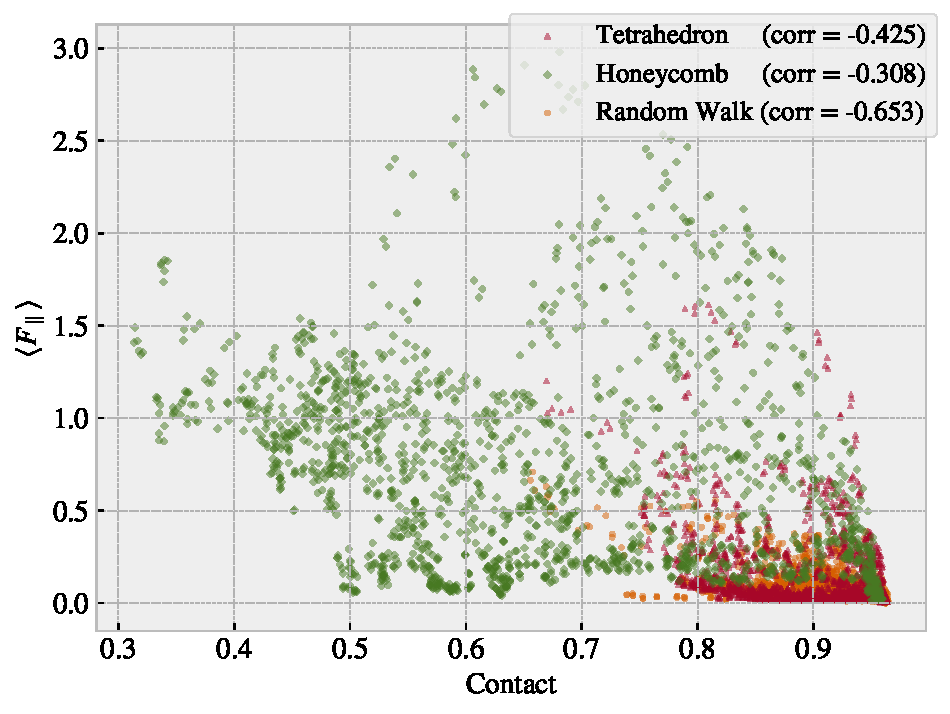
\includegraphics[width=\textwidth]{figures/ML/corr_contact_Ff.pdf}
      \caption{}
      % \label{fig:}
  \end{subfigure}
  \hfill
  \begin{subfigure}[t]{0.49\textwidth}
      \centering
      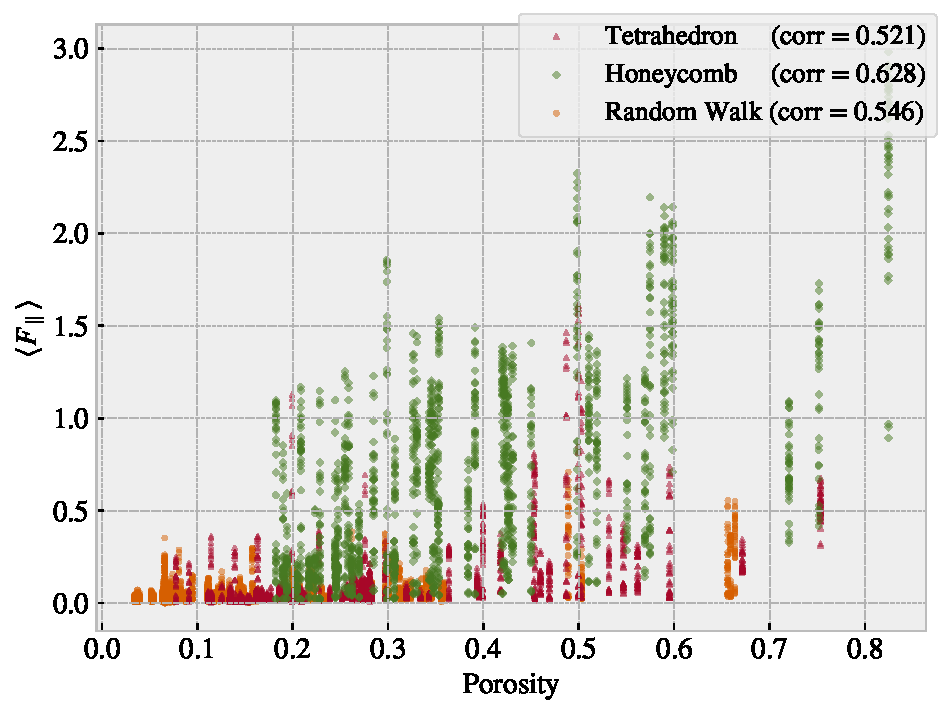
\includegraphics[width=\textwidth]{figures/ML/corr_porosity_Ff.pdf}
      \caption{}
      % \label{fig:}
  \end{subfigure}
  \hfill
     \caption{Scatter plot of the data sets Tetrahedron, Honeycomb and Random Walk (excluding the pilot study) for various variable combinations in order to visualize some chosen  correlations of interest and distributions in the data}
     \label{fig:corr_vis}
\end{figure}


\section{Properties of interest} 
In the pilot study (\cref{chap:pilot_study}) we found promising results for the idea of achieving a negative friction coefficient under the assumption of a system with coupled normal force and stretch. Hence, we will consider this as a main property of interest for our further exploration. However, it is not obvious how one should rigorously quantify this. The friction coefficient is by our definition (\cref{eq:mu_def2}) given as the slope of the friction $F_f$ vs.\ normal force $F_N$ curve. Hence, for two data points $\{(F_{N,1}, F_{f,1}), (F_{N,2}, F_{f,2})\}$, $F_{N,1} < F_{N,2}$ we can evaluate the associated friction coefficient $\mu_{1,2}$ as 
\begin{align*}
  \mu_{1,2} = \frac{F_{f,2} - F_{f,1}}{F_{N,2} - F_{N,1}} = \frac{\Delta F_f}{\Delta F_N}.
\end{align*}
In the pilot study, it became clear that the effects of friction under the
change of load is negligible in comparison to the effects related to stretch $S$.
Thus, by working under the assumption $F(F_N, S) \sim F(S)$ and a coupling $F_N
\propto R\cdot S$ with linear coupling ratio $R$ we get 
\begin{align}
  \mu_{1,2}(S_1, S_2) = \frac{\Delta F_{f}(S_1, S_2)}{R(S_2 - S_1)} \propto \frac{\Delta F_{f}(S_1, S_2)}{\Delta S}.
  \label{eq:mu_stretch}
\end{align}
With this reasoning we can in practice exchange $F_N$ with $S$ in the expression
for the friction coefficient of our coupled system. This justifies the search
for a strong negative slope on the friction vs.\ stretch curve as it can be
related to a negative friction coefficient in our proposed coupled system. The
remaining question is how to evaluate the strength of this property. By
definition, the minimum (most negative) slope value would give the lowest
friction coefficient. However, two data points with a small $\Delta S$,
corresponding to a small denominator in \cref{eq:mu_stretch}, would potentially
lead to a huge negative slope value without any significant decrease in
friction. Hence, we choose to consider the drop in friction with increasing
stretch as a better metric. For a given friction vs.\ stretch curve, we can
locate the local maxima and evaluate the difference to the succeeding local
minima. The biggest drop will serve as our indicator for a negative friction
coefficient. In this evaluation, we do not guarantee a monotonic decrease of
friction in the range of the biggest drop, but when searching among multiple
configurations this is considered a decent strategy to highlight configurations
of interest worthy of further investigation. In addition to the biggest drop in
friction, max drop, we also consider the minimum, $\min F_{\text{fric}}$, and
maximum, $\min F_{\text{fric}}$, friction along with the maximum difference
$\max \Delta f_{\text{fric}} = \max F_{\text{fric}} - \min F_{\text{fric}}$. The
extrema of these four properties for each of the designs categories
(Tetrahedron, Honeycomb and Random walk) and the Pilot study are summarized in
\cref{tab:data_properties} with the corresponding stretch profiles and
configurations shown in \crefrange{fig:PP_min}{fig:PP_max_drop} (excluding the
pilot study). The stretch profiles for the full dataset are shown in appendix
\cref{sec:data_stretch_profiles}. 

From the property comparison in \cref{tab:data_properties} we see in general that the Honeycomb pattern is superior in terms of the maximum properties which aligns with the pilot study results as well. However, by including more variations of the patterns we find an improvement in the max drop category for both the Tetrahedron pattern ($0.5098 \to 0.8841$) and the Honeycomb pattern ($0.9674 \to 1.2785$). The comparison also reveals that the non-cut sheet is still the best candidate for a low friction behavior which indicates that the Kirigami designs cannot be used to further reduce friction in our simulation domain. The Random walk property scores are in general on a comparable order of magnitude which indicates that these randomized patterns have some relevance concering the usage as training data.

\hl{Perhaps comment a bit on what the Random walk top candidates tell about the optimization for the different properties?}

\begin{table}[H]
  \begin{center}
  \caption{Evaluation of the properties of interest for our dataset.}
  \label{tab:data_properties}
  \begin{tabular}{| c | c | c | c|} \hline
  \textbf{Tetrahedron} & Configuration & Stretch & Value [nN]  \\ \hline
  $\min F_{\text{fric}}$ & $(3,9,4)$ &  0.0296 & 0.0067 \\ \hline
  $\max F_{\text{fric}}$ & $(5,3,1)$ & 0.1391 & 1.5875 \\ \hline
  $\max \Delta F_{\text{fric}}$  & $(5, 3, 1)$ & $[0.0239, 0.1391]$ & 1.5529 \\ \hline
  max drop & $(5,3,1)$ & $[0.1391, 0.1999]$ & 0.8841 \\ \hline
  \multicolumn{4}{c}{} \\ \hline
  % \textbf{Tetrahedron} & \multicolumn{3}{c|}{} \\ \hline
  \textbf{Honeycomb} & Configuration & Stretch & Value [nN]  \\ \hline
  $\min F_{\text{fric}}$ & $(2, 5, 1, 1)$ &  0.0267 & 0.0177 \\ \hline
  $\max F_{\text{fric}}$ & $(2, 1, 1, 1)$ & 1.0654 & 2.8903 \\ \hline
  $\max \Delta F_{\text{fric}}$  & $(2, 1, 5, 3)$ & $[0.0856, 1.4760]$ & 2.0234 \\ \hline
  max drop & $(2, 3, 3, 3)$ & $[0.5410, 1.0100]$ & 1.2785 \\ \hline
  \multicolumn{4}{c}{} \\ \hline
  \textbf{Random walk} & Configuration & Stretch & Value [nN]  \\ \hline
  $\min F_{\text{fric}}$ & 12 &  0.0562 & 0.0024\\ \hline
  $\max F_{\text{fric}}$ & 96 & 0.2375 & 0.5758 \\ \hline
  $\max \Delta F_{\text{fric}}$  & 96 & $[0.0364, 0.2375]$ & 0.5448 \\ \hline
  max drop & 01 & $[0.0592, 0.1127]$ & 0.1818 \\ \hline
  \multicolumn{4}{c}{} \\ \hline
  \textbf{Pilot study} & Configuration & Stretch & Value [nN]  \\ \hline
  $\min F_{\text{fric}}$ & No cut & 0.2552 & 0.0012 \\ \hline
  $\max F_{\text{fric}}$ & Honeycomb & 0.7279 & 1.5948 \\ \hline
  $\max \Delta F_{\text{fric}}$  & Honeycomb & 0.7279 & 1.5325 \\ \hline
  max drop & Honeycomb & $[0.7279, 1.0463]$ & 0.9674 \\ \hline
\end{tabular}
\end{center}
\end{table}



\begin{figure}[H]
  \centering
  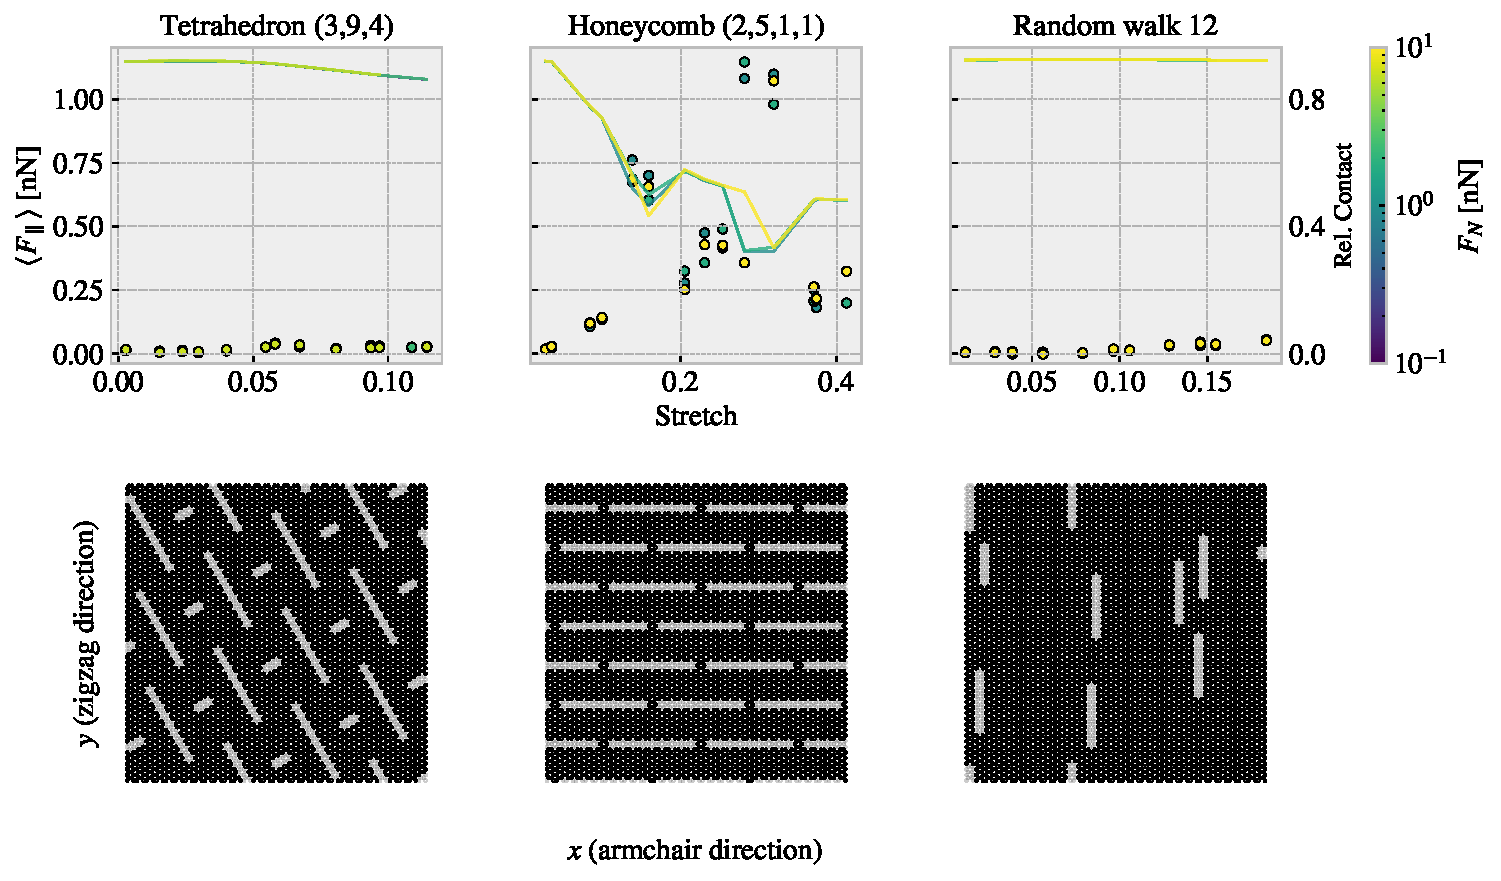
\includegraphics[width=\linewidth]{figures/stretch_profiles/PP_min.pdf}
  \caption{Minimum friction: Configurations corresponding to the minimum friction.}
  \label{fig:PP_min}
\end{figure}


\begin{figure}[H]
  \centering
  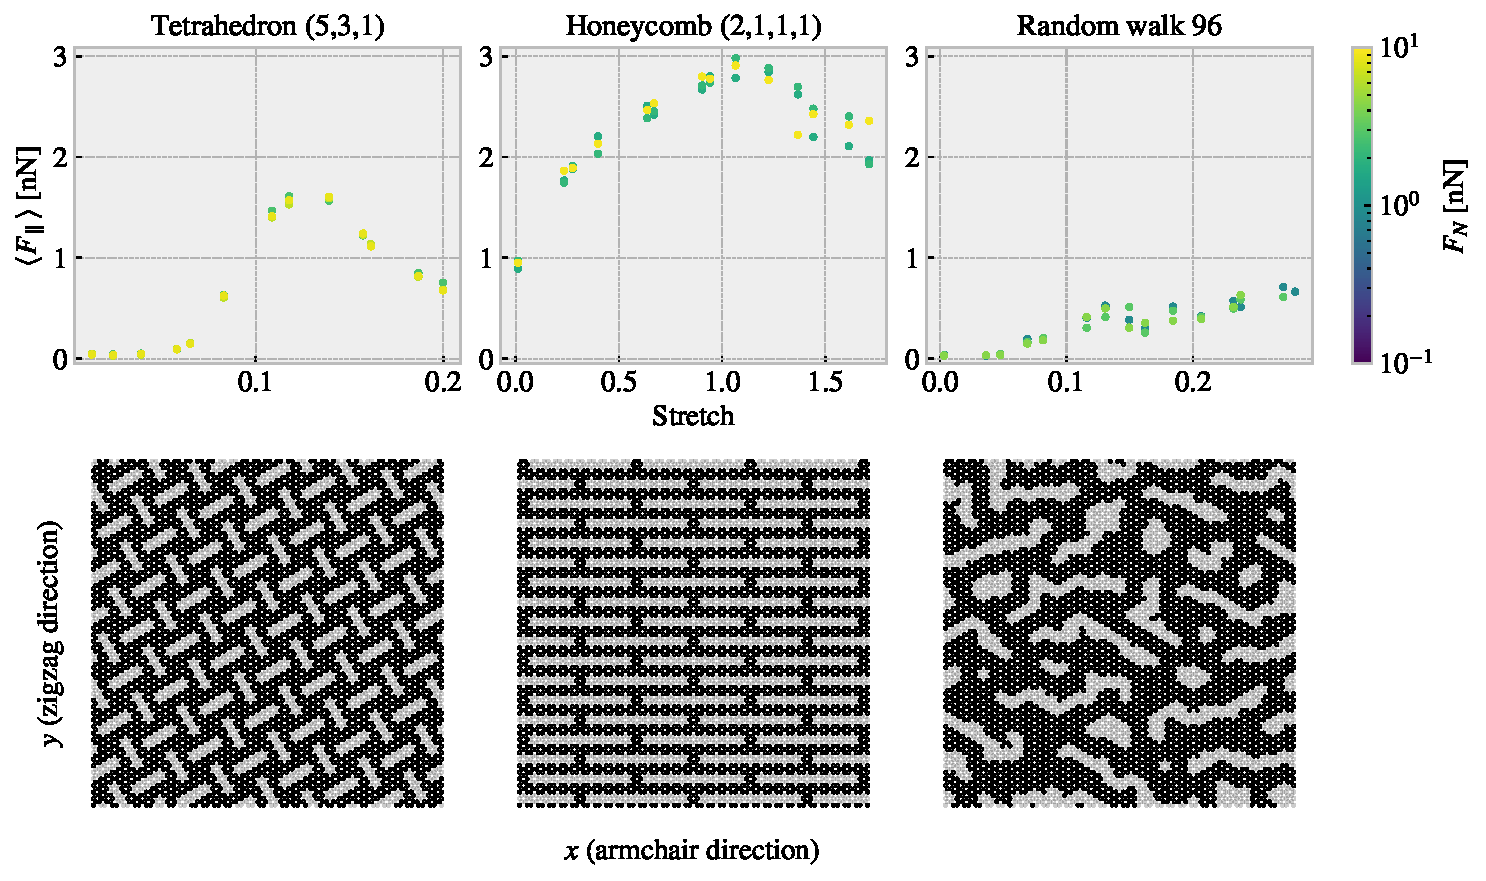
\includegraphics[width=\linewidth]{figures/stretch_profiles/PP_max.pdf}
  \caption{Maximum friction: Configurations corresponding to the maximum friction.}
  \label{fig:PP_max}
\end{figure}


\begin{figure}[H]
  \centering
  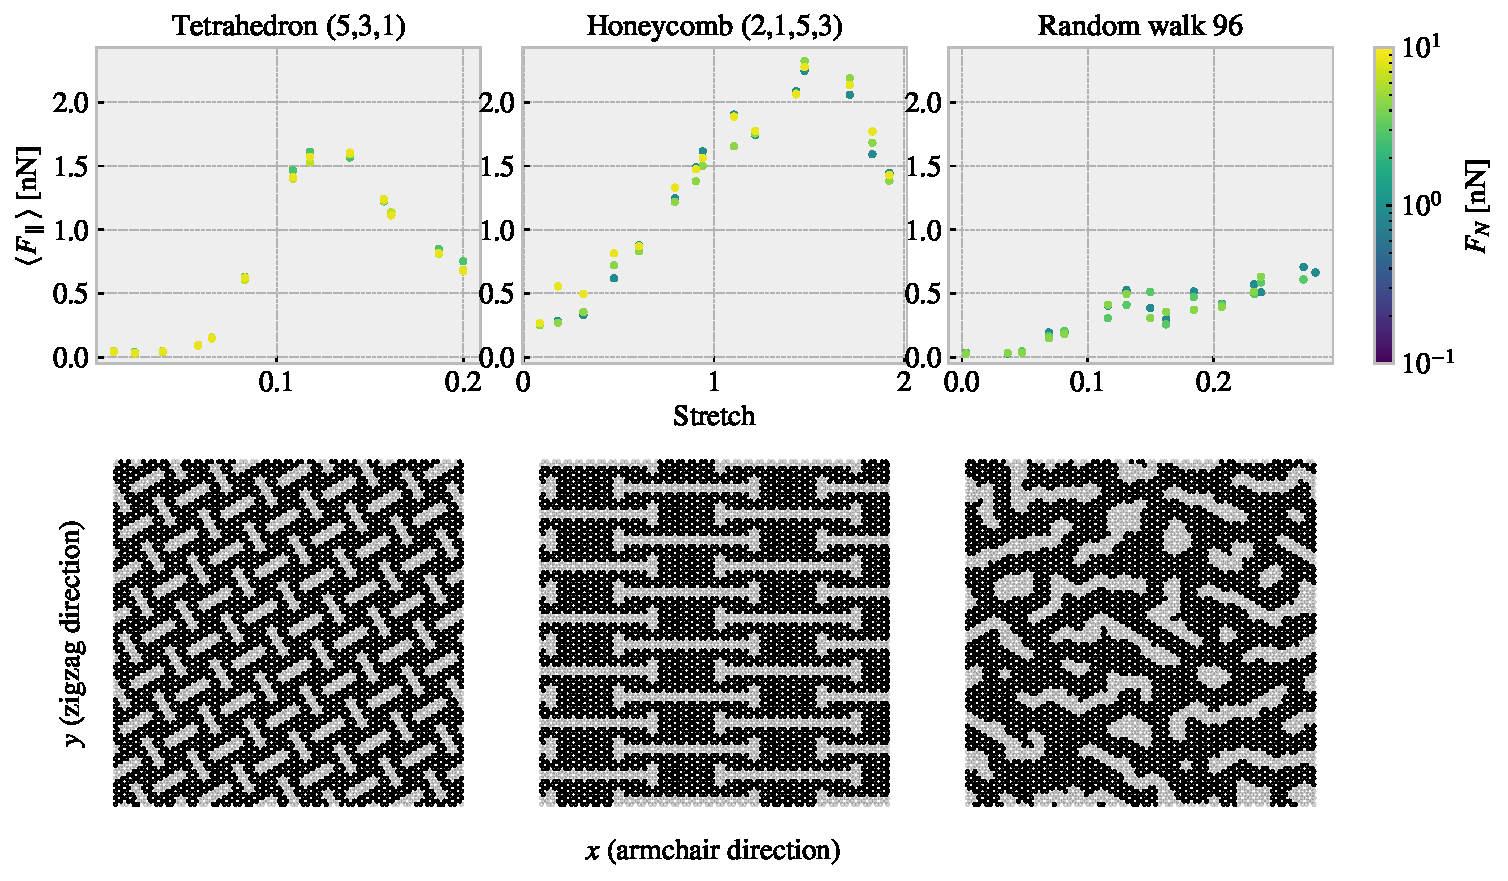
\includegraphics[width=\linewidth]{figures/stretch_profiles/PP_max_diff.pdf}
  \caption{Maximum Difference: Configurations corresponding to the biggest difference in friction in the dataset for each pattern.}
  \label{fig:PP_max_diff}
\end{figure}  

\begin{figure}[H]
  \centering
  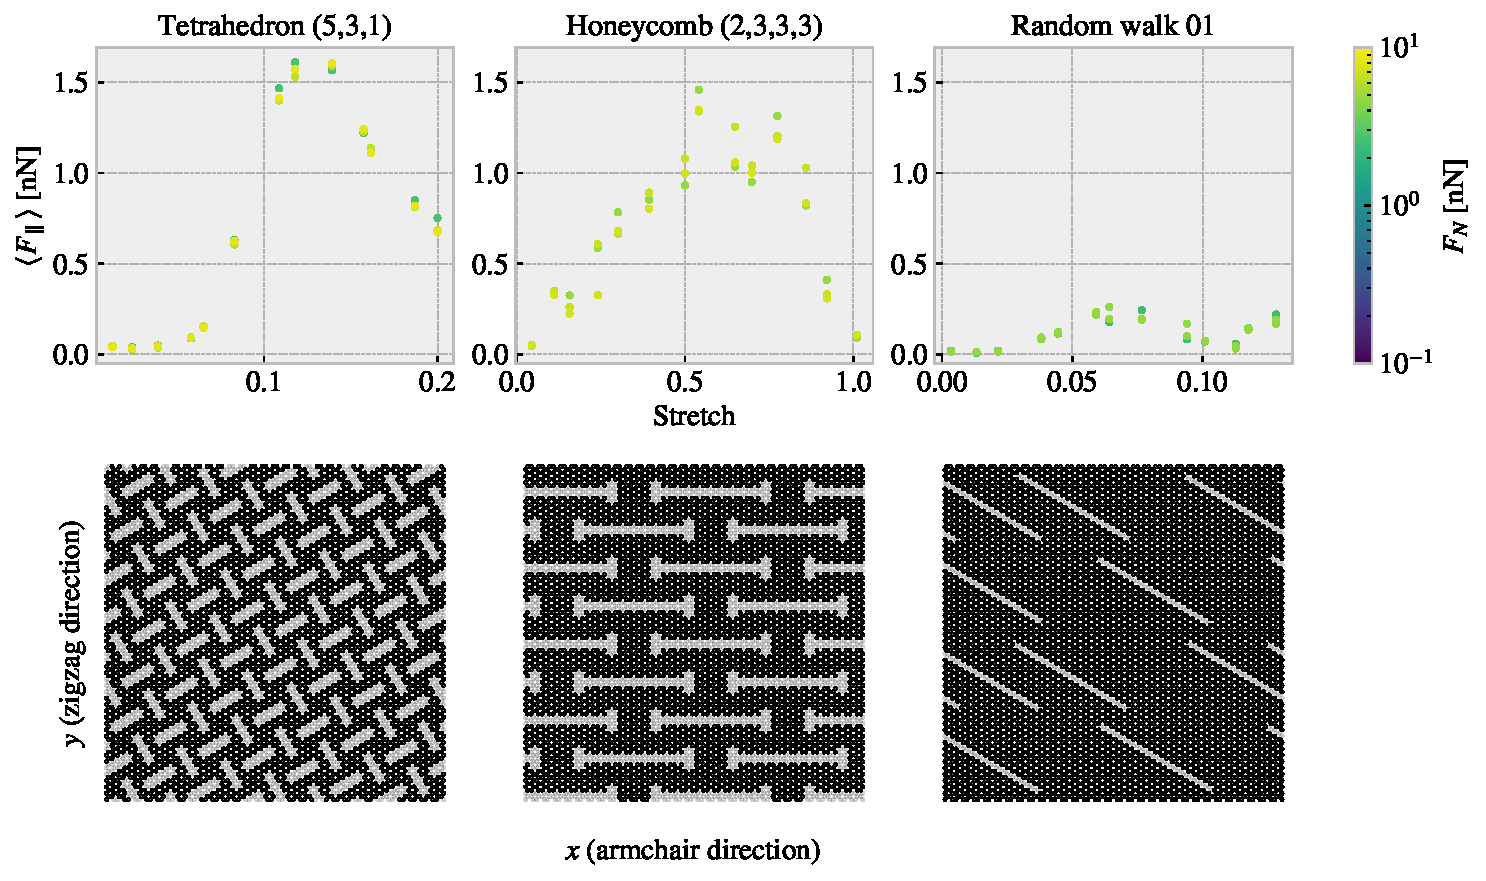
\includegraphics[width=\linewidth]{figures/stretch_profiles/PP_max_drop.pdf}
  \caption{Maximum drop: Configuratiosn corresponding to the biggest friction drop in the dataset for each pattern.}
  \label{fig:PP_max_drop}
\end{figure}  





% \begin{figure}[H]
%   \centering
%   \begin{subfigure}[t]{0.49\textwidth}
%       \centering
%       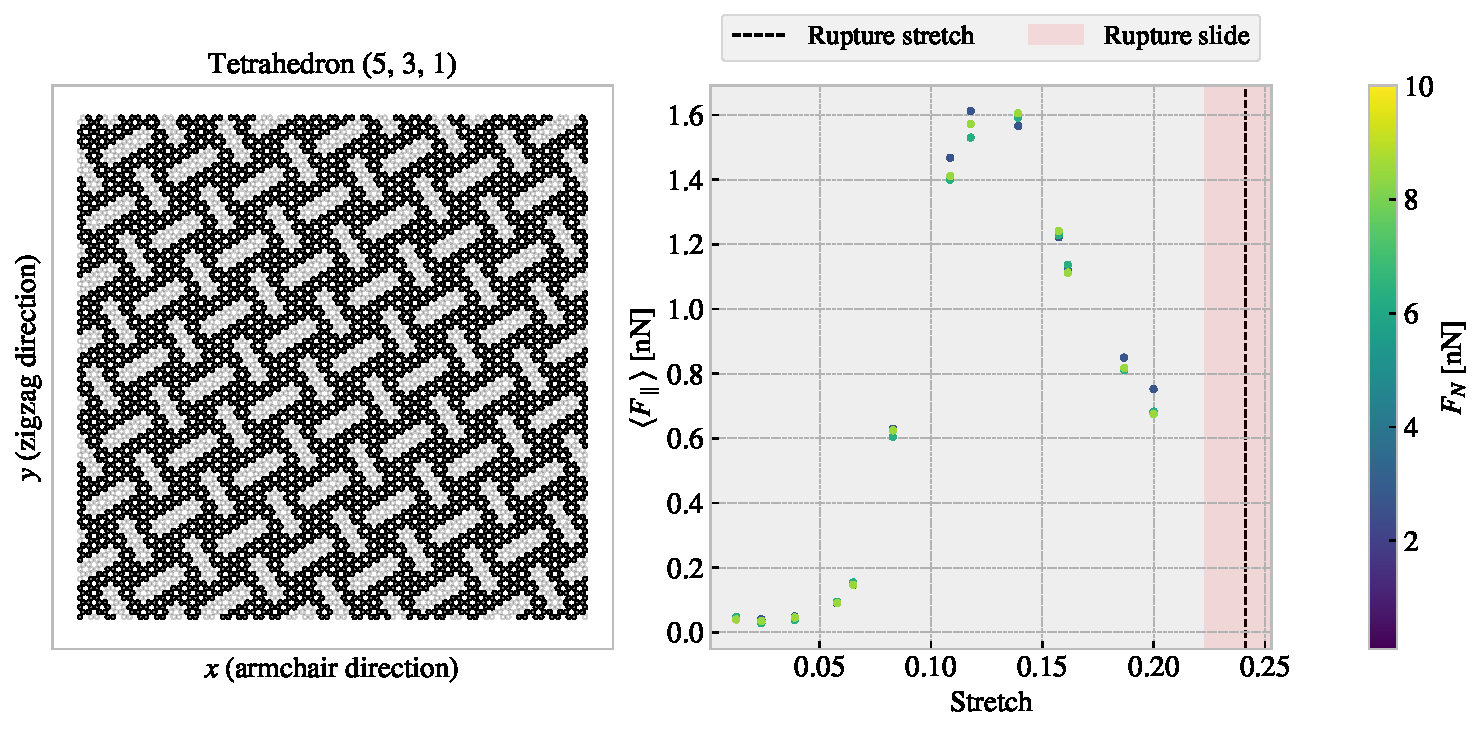
\includegraphics[width=\textwidth]{figures/stretch_profiles/PP_pop_27.pdf}
%       \caption{}
%   \end{subfigure}
%   \hfill
%   \begin{subfigure}[t]{0.49\textwidth}
%       \centering
%       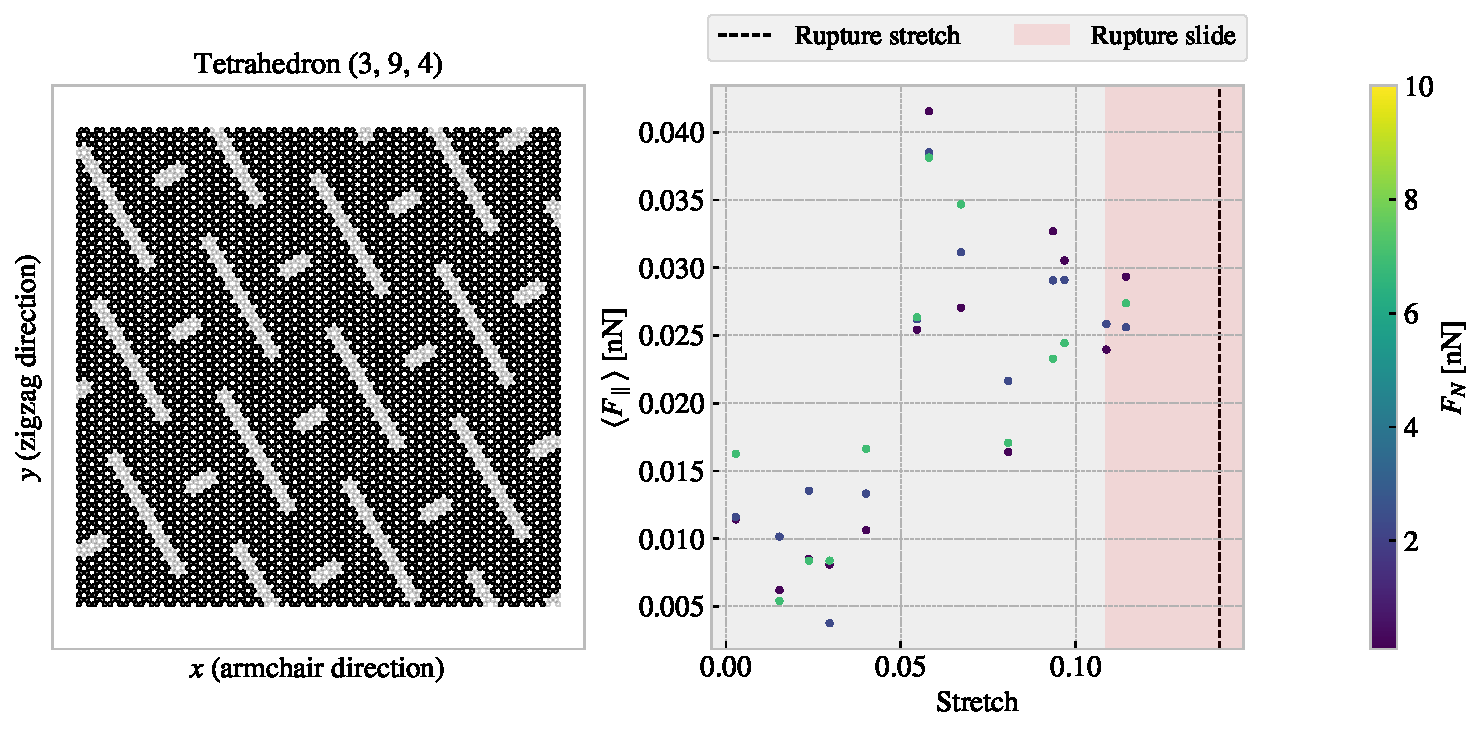
\includegraphics[width=\textwidth]{figures/stretch_profiles/PP_pop_31.pdf}
%       \caption{}
%   \end{subfigure}
%   \hfill
%   \begin{subfigure}[t]{0.49\textwidth}
%       \centering
%       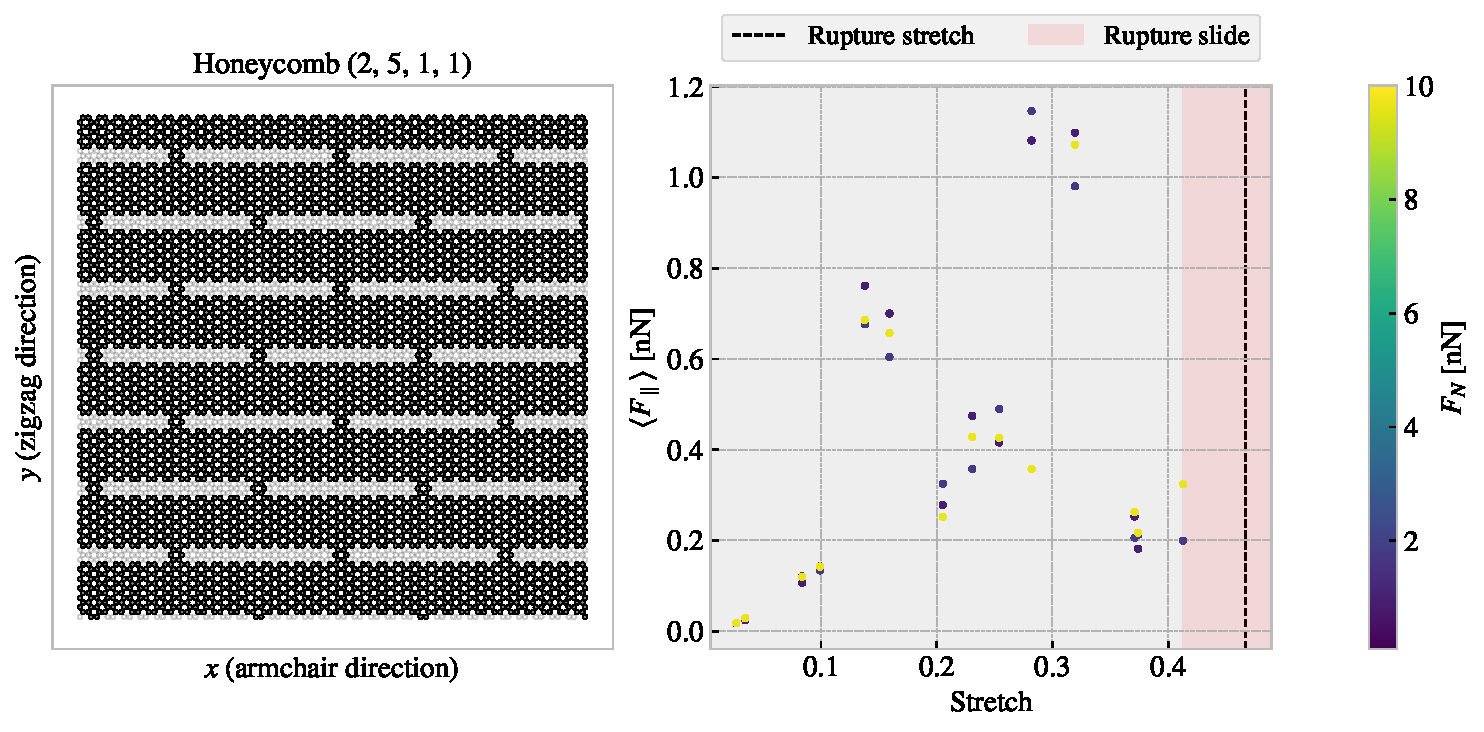
\includegraphics[width=\textwidth]{figures/stretch_profiles/PP_hon_6.pdf}
%       \caption{}
%   \end{subfigure}
%   \hfill
%   \begin{subfigure}[t]{0.49\textwidth}
%       \centering
%       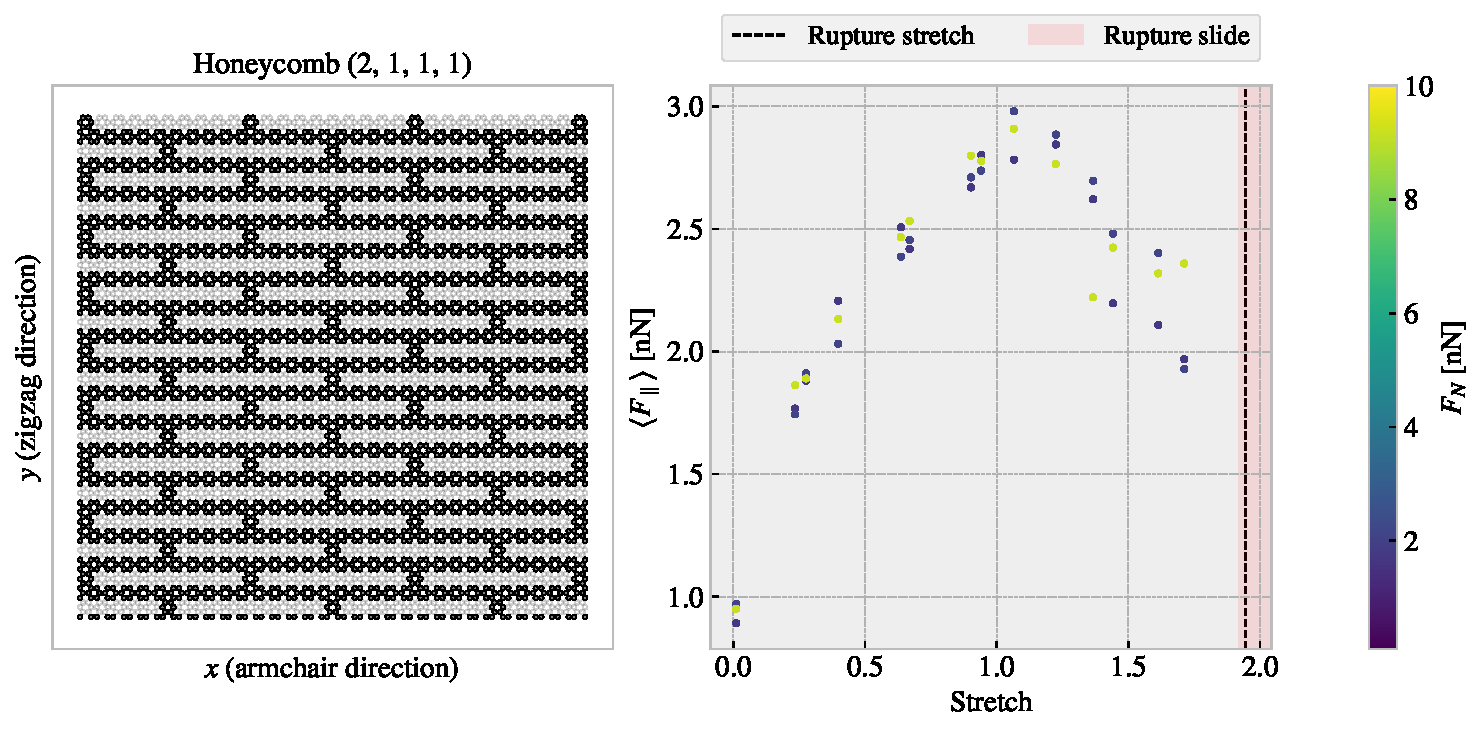
\includegraphics[width=\textwidth]{figures/stretch_profiles/PP_hon_12.pdf}
%       \caption{}
%   \end{subfigure}
%   \hfill
%   \begin{subfigure}[t]{0.49\textwidth}
%       \centering
%       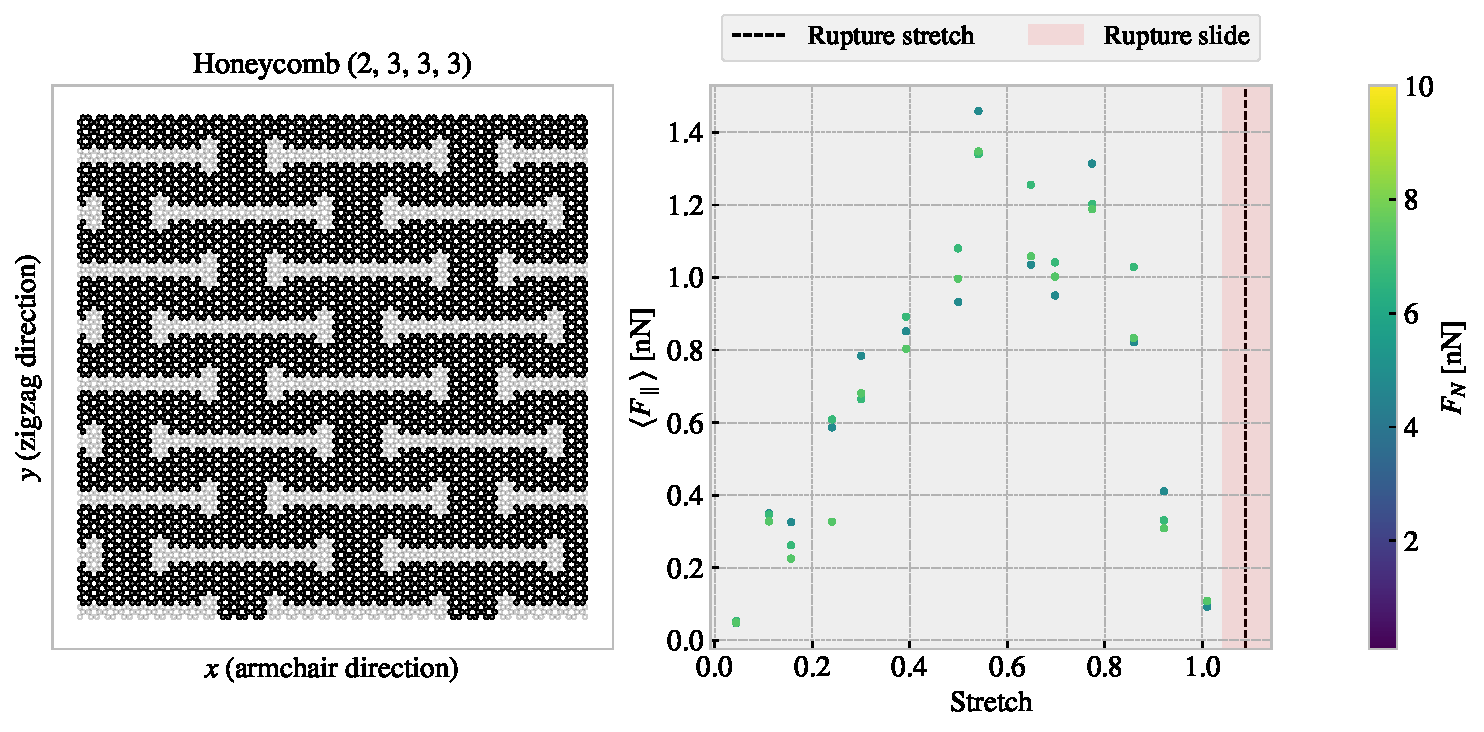
\includegraphics[width=\textwidth]{figures/stretch_profiles/PP_hon_28}
%       \caption{}
%   \end{subfigure}
%   \hfill
%   \begin{subfigure}[t]{0.49\textwidth}
%       \centering
%       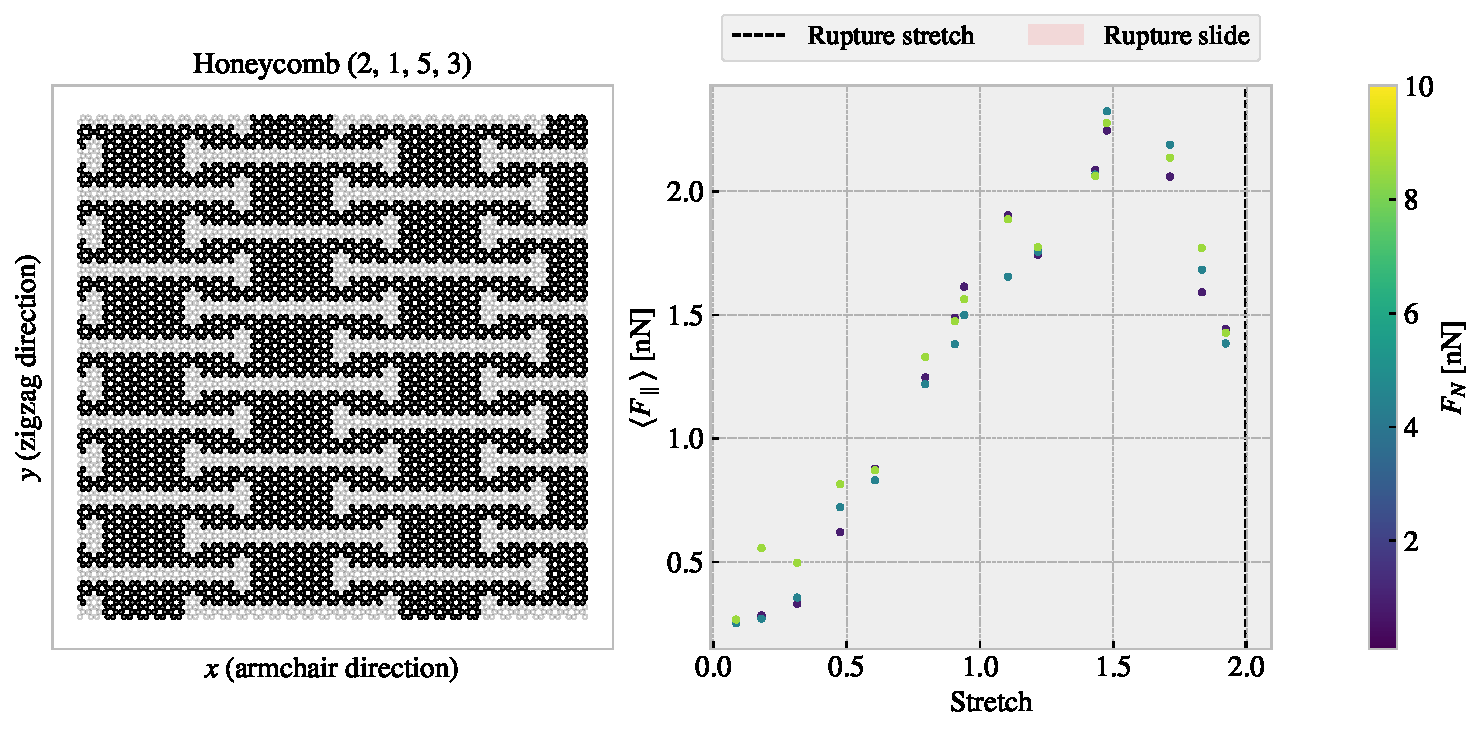
\includegraphics[width=\textwidth]{figures/stretch_profiles/PP_hon_42.pdf}
%       \caption{}
%   \end{subfigure}
%   \hfill
%   \begin{subfigure}[t]{0.49\textwidth}
%       \centering
%       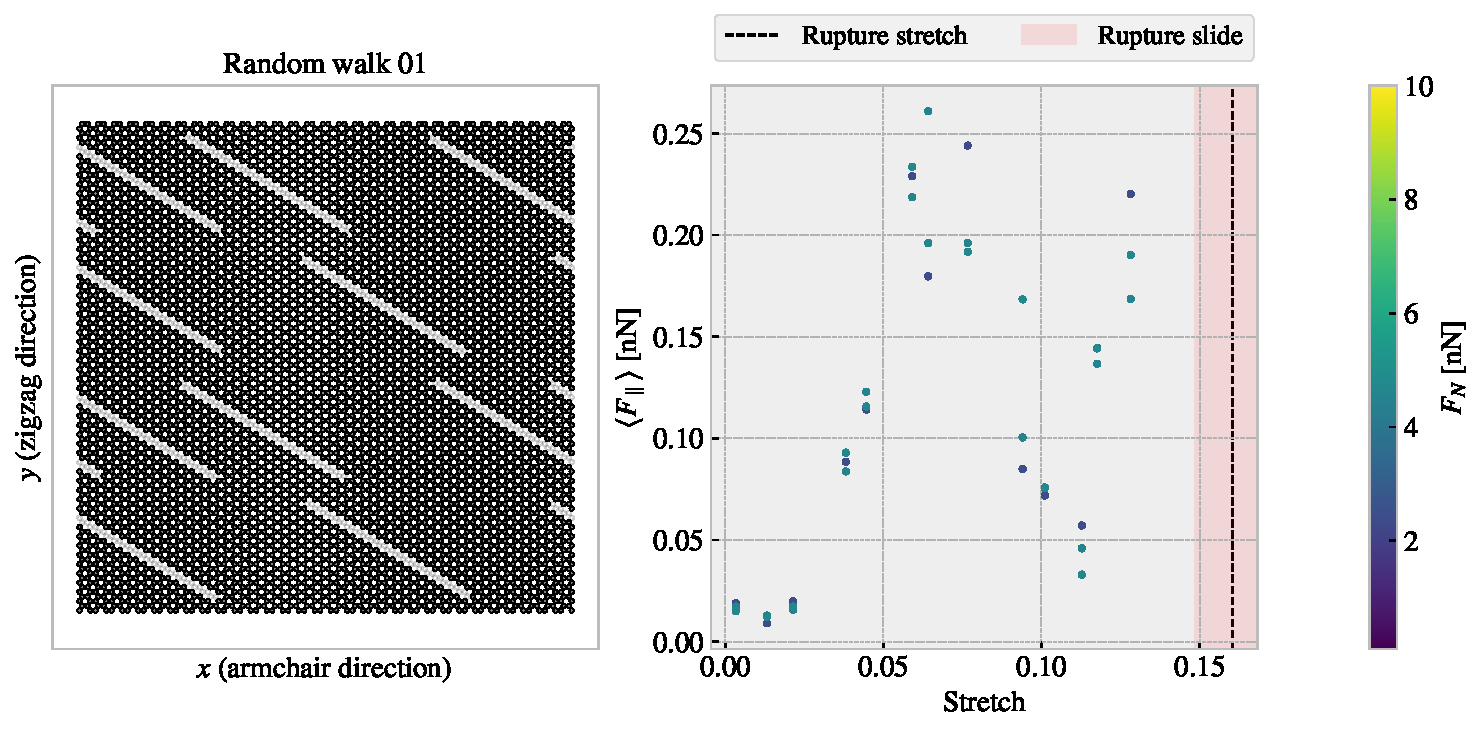
\includegraphics[width=\textwidth]{figures/stretch_profiles/PP_RW01.pdf}
%       \caption{}
%   \end{subfigure}
%   \hfill
%   \begin{subfigure}[t]{0.49\textwidth}
%       \centering
%       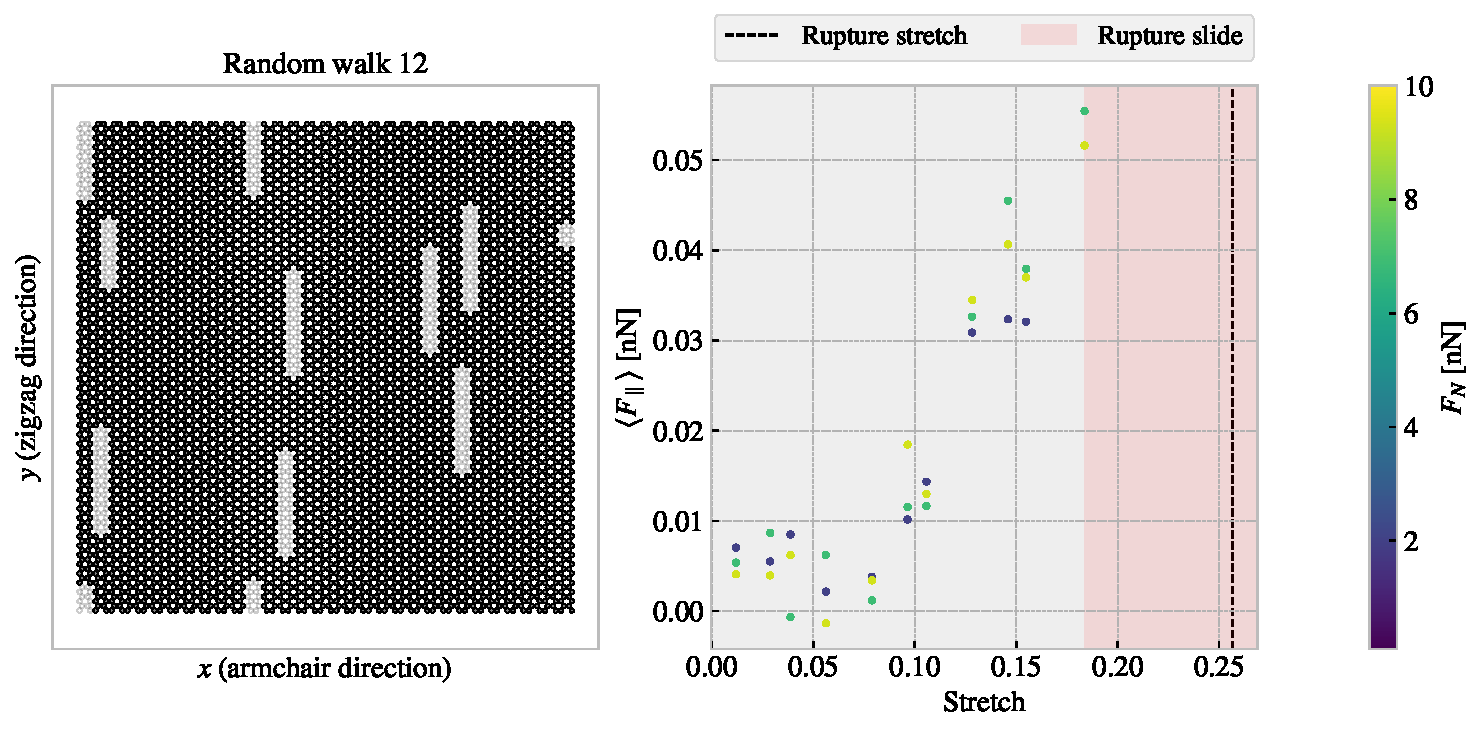
\includegraphics[width=\textwidth]{figures/stretch_profiles/PP_RW12.pdf}
%       \caption{}
%   \end{subfigure}
%   \hfill
%   \begin{subfigure}[t]{0.49\textwidth}
%       \centering
%       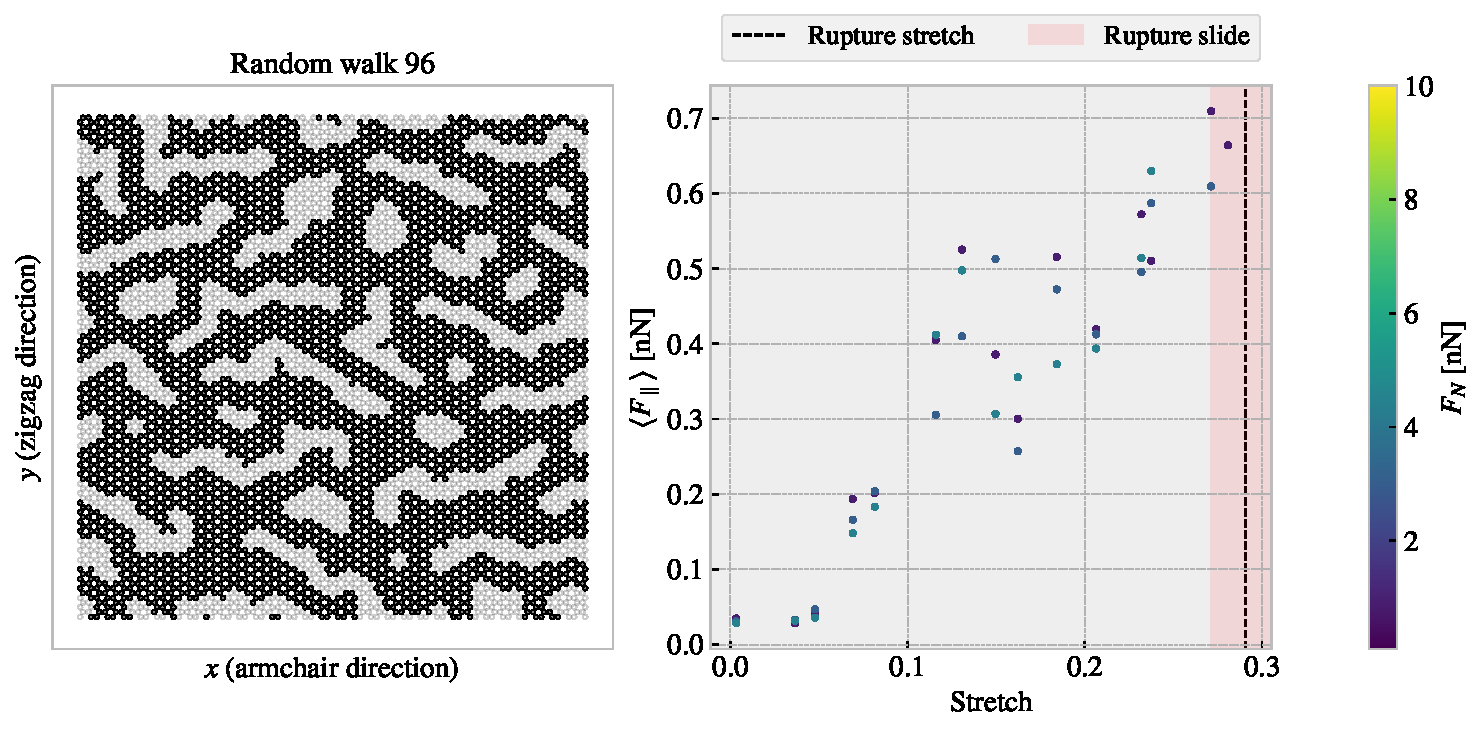
\includegraphics[width=\textwidth]{figures/stretch_profiles/PP_RW96.pdf}
%       \caption{}
%   \end{subfigure}
%   \hfill
%      \caption{}
%      \label{fig:}
% \end{figure}








\section{Machine learning}

Given the \acrshort{MD}-based datset we investigate the possibilities of training a machine learning model to predict the friction behaviour from a given Kirigami configuration, stretch and load. 


% General stuff to include. Remember to talk about batchnorm, optimizer, stopping at best epoch. 


\subsection{Architecture}
Due to the spatial dependencies in the Kirigami configurations, we use a convolutional neural network (\acrshort{CNN}) for our model architecture. Similar studies which predict mechanical properties for graphene sheets have used a VGGNet style network, Hanakata et al.\ \cite{PhysRevLett.121.255304, PhysRevResearch.2.042006} and Wan et al.\ \cite{graphene/hBN}, which we adopt for this study as well. The VGGNet-16 architecture illustrated in \cref{fig:VGGNet16} shows the key features that we will include:
\begin{itemize}
  \item The image is processed through a series of $3 \times 3$ convolutional filters (the smallest size capable of capturing spatial dependencies) using a stride of 1 with an increasing number of channels throughout the network. Each convolutional layer is followed by a ReLU activation function. 
  \item The spatial dimensions are reduced by a max pooling, filter size $2 \times 2$ and a stride of 2, which halfs the spatial resolution each time. 
  \item The latter part of the network consists of a fully connected part followed by a ReLU activation. The transition from the convolutional to the fully connected part is achieved by applying a filter with the same dimensions as the last convolutional feature map. This essentially maps the spatial output to the fully connected layer with the number of channels corresponding to the nodes in this layer.
\end{itemize}

\begin{figure}[H]
  \centering
  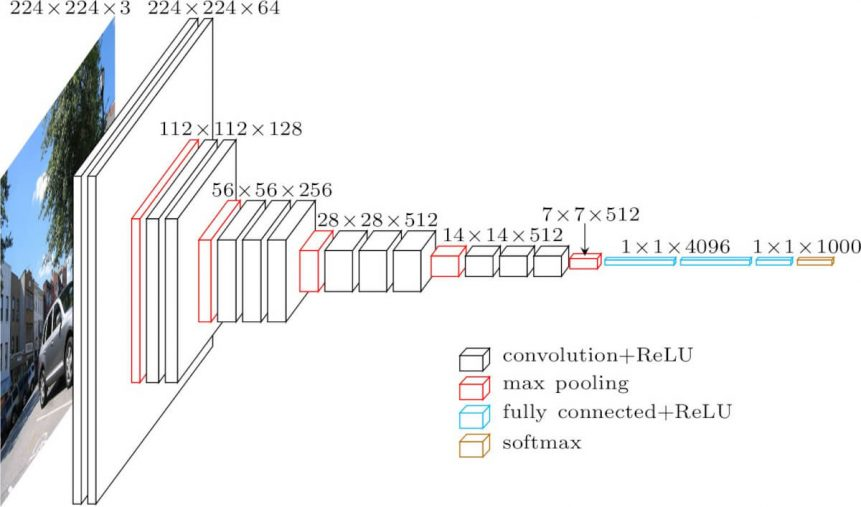
\includegraphics[width=0.7\linewidth]{figures/ML/VGGNet16.jpg}
  \caption{VGGNet 16. Source \url{https://neurohive.io/en/popular-networks/vgg16/}.}
  \label{fig:VGGNet16}
\end{figure}

We deviate from the VGGNet-16 architecture by including batch normalization and restricting ourselves to build the convolutional part in terms of the blocks: (Convolution $\to$ Batch normalization $\to$ ReLU $\to$ Max pooling). Similarly, we define a fully connected block by two elements (Fully connected $\to$ ReLU) which match the VGGNet model. Hanakata et al.\ and Wan et al.\ used a similar architecture with the parameters 
\begin{align*}
  \text{Hanakata et al.\ \cite{PhysRevLett.121.255304}} & \qquad C16 \ C32 \ C64 \ D64, \\ 
  \text{Wan et al.\ \cite{graphene/hBN}} & \qquad C16 \ C32 \ D32 \ D16,
\end{align*}
Where $C$ denotes a convolutional block with the number denoting the number of channels, and $D$ a fully connected (dense) block with the number denoting number of nodes. For the process of determining a suiting complexity for the architecture, we adopt the approach by Wan et al.\ \cite{graphene/hBN} who used a ``staircase'' pattern for combining convolutional and fully connected blocks. By defining a starting number of channels $S$ and network depth $D$ we fill the first half with convolutional blocks doubling in channel number for each layer and the latter half with fully connected blocks having the number of nodes decreasing in a reverse pattern. For instance the architecture $S4D8$ will take the form
Following this pattern a $(S=4, D=8)$ would take the form
\begin{align*}
  \text{Input} \to \underbrace{\overbrace{C4}^{S \ = \ 4}C8 \ C16 \ C32 \ D32 \ D16 \ D8 \ D4}_{D \ = \ 8} \to \text{Output}.
\end{align*} 
This provides a simple description where $S$ and $S$  can be varied systematically for a grid search over architecture complexity. 


\subsection{Data handling}
\subsubsection{Input}
We use three variables as input: Kirigami configuration, stretch of the sheet
and applied normal load. While the first is a two-dimensional input the latter
are both scalars. This gives rise to two main options for the data structure
\begin{enumerate}
  \item Expand the scalar values (stretch and load) into 2D matrices of the same
  size as the Kirigami configuration (copying the scaler value to all positions). This can then be merged into an image of three channels used as a single input.  
  \item Pass only the Kirigami configuration through the convolutional part of the network and introduce the remaining scalar values into the fully connected part of the network halfway in. 
\end{enumerate}
Both options utilize the same data, but the first is more appropriate if the configuration should be considered in context with the applied stretch and load, while the latter corresponds to a more independent processing. We implemented both options but it was immediately clear from the test runs that option 1 was producing the most promising result which we settled on.

\subsubsection{Output}
For the output we are mainly concerned with mean friction and the rupture
detection. In combination, this will make the model able to produce a friction vs.\ stretch curve with an estimated stopping point as well. However, for some cases, the model can benefit from having additional output variables to adjust for \hl{source}, and thus we include we include maximum friction, contact, porosity and rupture stretch in the output as well. This also gives us more options for exploring the relationship in the data later on. Notice that we weight the importance of these output variables different in the loss as described in 
variables differently as described in \cref{sec:loss}. 
\\
\\
\hl{Removed this part, do you think it has any relevance: Notice that the rupture stretch refers to the value found in the rupture test without load, but as the sheet always ruptures before or just around this point in a loaded state this provides some information for the training to lean on, even though it is in the output state. In principle, we could add a penalty whenever the network predicts the sheet to be attached for stretch values above the rupture stretch, but we found the performance of the rupture prediction to be satisfactory without such penalties.}


\subsubsection{Data augmentation}
In order to increase the utility of the available data one can introduce data augmentation. For most classification tasks this usually includes distortions such as color shifts, zoom, flip etc. However, such distortions are only valid since the classification network should still classify a cat as a cat even though it is suddenly a bit brighter or flipped upside down. For our problem, we can only use augmentation that matches a physical symmetry. Such a symmetry exists for reflection across the y-axis. We cannot do this across the
x-axis as the sheet is translated in a positive y-direction meaning that the reflected version would correspond to a change in the sliding direction which we cannot expect to be fully symmetric. 

% We definitely expect a snow plow to perform differently when attached in reverse and thus by analogy we would expect the direction of sliding with respect to the configuration to be of importance. 

\subsection{Loss}\label{sec:loss}
The output contains two different types of variables: scalar values and binary values (0: False 1: True). For the scalar values we use the Mean Squared Error (\acrshort{MSE})
\begin{align*}
  L_{\text{MSE}} = \frac{1}{N} \sum_{i = 1}^N (y_i - \hat{y}_i)^2,
\end{align*}
where $N$ is the number of data entries, $y$ are the true output and
$\hat{y}$ are the predicted values. For the binary output, we use binary cross entropy 
\begin{align*}
  L_{\text{BCE}} = -\frac{1}{N} \left[\sum_{i = 1}^N [t_i\log{(p_i)} + (1-t_i)\log{(1 - p_i)}]\right],
\end{align*}
where $t\in \{0,1\}$ is the truth label. \hl{Does this belong in theory
entirely? I do introduce it there but I guess I have to mention the choice here still}. We calculate the total loss as a weighted sum of the loss associated with
each variable
\begin{align*}
  L_{tot} = \sum_{v} W_v\cdot L_v.
\end{align*}
We choose the weights to be $1/2$ for the mean friction and $1/10$ for the
remaining 5 variables, thus sharing the loss evenly for the remaining 50\% of the weight. During the introductory phase of the training, we tried different settings for these weights. We found that the results varied little and concluded that the training is not very sensitive to this choice, for which we stuck with the values defined above.

\subsection{Hypertuning}
% Show overfitting curve for some of the training results?
For the hypertuning we focus on architecture complexity, learning rate, momentum and weight decay. Thus the non-chaning elements are the use of the ADAM optimizer with the initial default values of $beta_1 = 0.9, \beta_2 = 0.999$ and zero weight decay (we will change momentum $\beta_1$ and weight decay). We use a batch size of 32 and train the model for a maximum of 1000 epochs, but we save the best model during training based on the lowest validation loss. 

Since the learning rate is considered to be one of the most important hyperparameters we will determine a suitable choice for the learning rate using the learning rate range test for each of the two major grid searches:
\begin{enumerate}
  \item Architecture complexity grid search of $S$ vs.\ $D$ with individually chosen learning rates for each complexity combination.
  \item Momentum vs.\ weight decay grid search with learning range chosen with regard to the momentum. 
\end{enumerate}
We consider first the architectures in the range $S \times D =
\{2,4,8,16,32,64,128,256\} \times \{4,6,8,10,12,14\}$. For each architecture
complexity, we perform an initial learning rate range test, increasing the
the learning rate until the training loss diverges. The suggested learning rate is then determined as the point for which the training loss decreases most rapidly. The learning rate is increased exponentially within the range \num{e-7} to 10 with increments for each training batch iteration. This is done for just a single epoch where a training batch size of 32 yields a total of 242 increments. This corresponds to an exponent increment of approximately $1/30$ giving a relative increase $10^{1/30} \sim 108\%$ per batch iteration. The learning rate range test is presented in \cref{fig:LR_range} for variours model architectures. We notice that the suggested learning rate decreases with an increasing number of model parameters. This decrease is further independent of the specific relationship between $S$ and $D$.

\begin{figure}[H]
  \centering
  \begin{subfigure}[t]{0.49\textwidth}
      \centering
      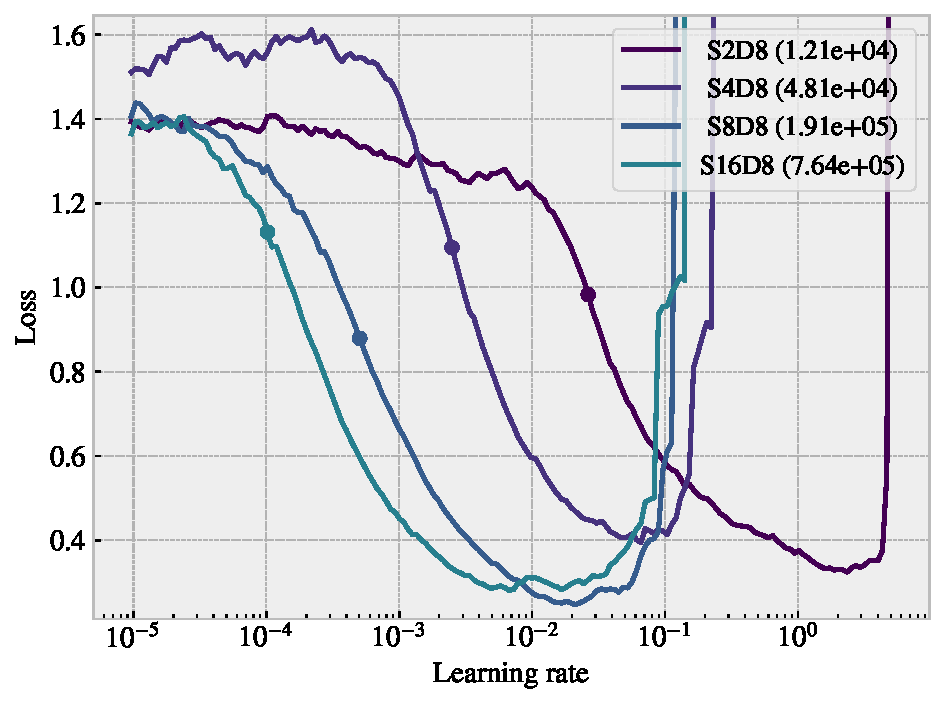
\includegraphics[width=\textwidth]{figures/ML/LR_range_specific.pdf}
      \caption{}
      % \label{fig:}
  \end{subfigure}
  \hfill
  \begin{subfigure}[t]{0.49\textwidth}
      \centering
      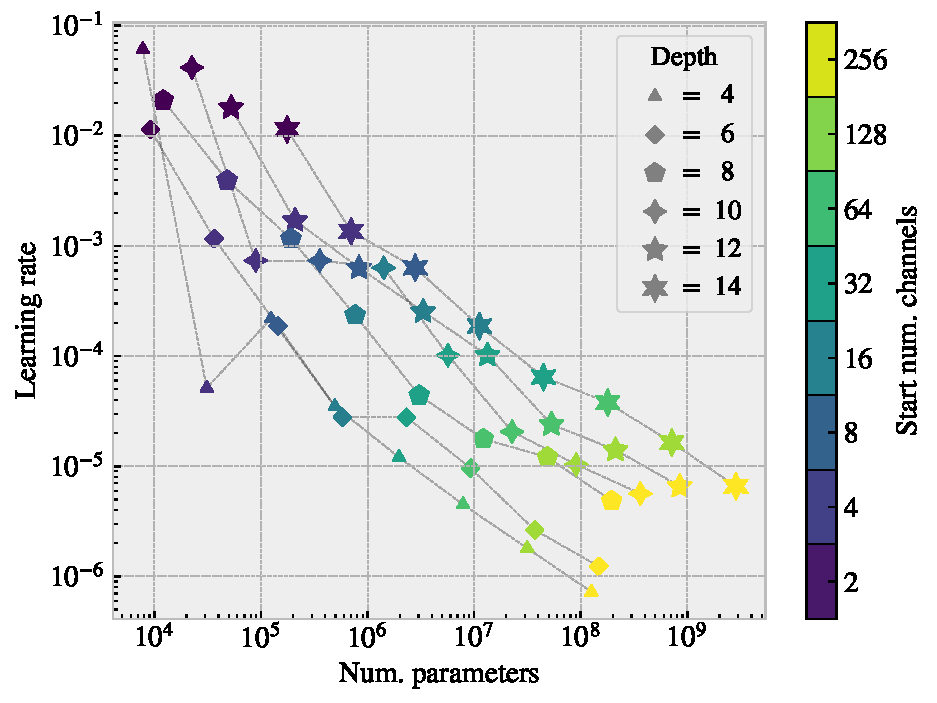
\includegraphics[width=\textwidth]{figures/ML/LR_range_full.pdf}
      \caption{}
      % \label{fig:}
  \end{subfigure}
  \hfill
  \caption{Learning rate range test for various model complexities. We increase the learning rate exponentially from num{e-7} to 10 during one epoch corresponding to an exponent increment of roughly $1/30$ per batch iteration. $(a)$ shows a few examples of the training loss history as a function of learning rate. The examplatory architectures are S[2, 16]D8 with the corresponding number of model parameters shown in parentheses in the legend. The dot indicates the suggested learning rate at the steepest decline of the slope. $(b)$ shows the full results of suggested learning rates depending on the number of model parameters with color coding differentiating the number of start channels and marker types differentiating different model depths. }
  \label{fig:LR_range}
\end{figure}
With the use of the suggested learning rates from \cref{fig:LR_range} we perform
a grid search over the corresponding $S$ and $D$ parameters. We evaluate both
the loss and the mean friction $R_2$ score for the validation data which is shown in \cref{fig:A_search_perf} together with the best epoch and the number of model
parameters. Additionally, we evaluate the mean friction $R_2$ score for a
selected set of configurations. This set consists of the top 10 configurations
with respect to maximum friction drop for the Tetrahedron and Honeycomb pattern
respectively. This is done as a way of evaluating the performance on the
non-linear stretch curves which we immediately found to be the more difficult patterns to capture. The selected evaluation is shown in \cref{fig:A_search_compare}. Note
that these patterns are already a part of the full dataset and thus the data points
related to these patterns are most likely present in both the training and the validation data set. Hence, the performance must be considered in conjunction with the actual validation performance in \cref{fig:A_search_perf}.

\begin{figure}[H]
  \centering
  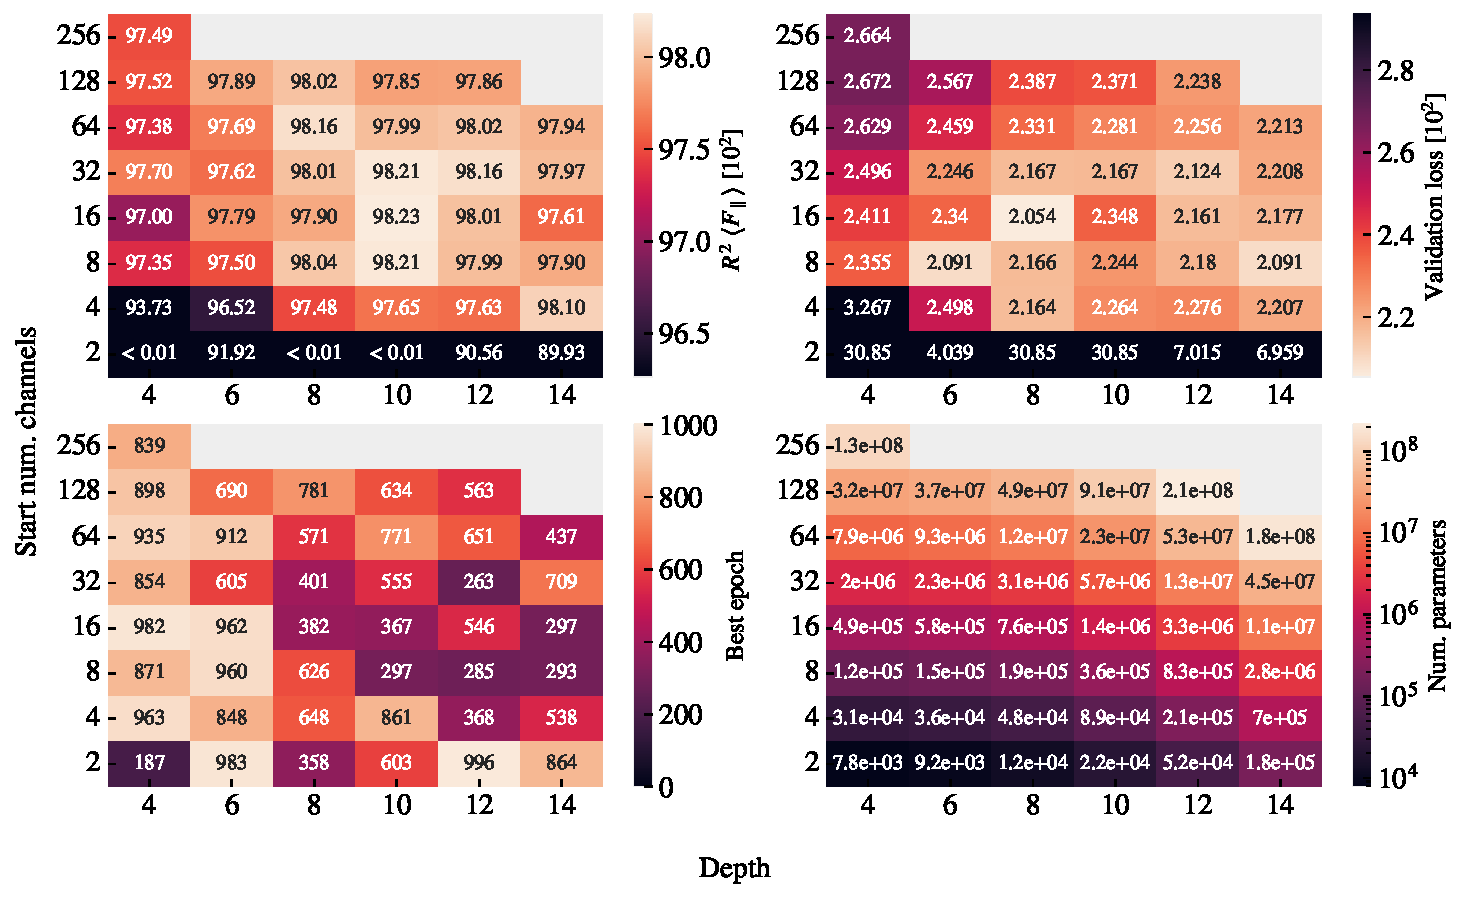
\includegraphics[width=\linewidth]{figures/ML/A_search_perf.pdf}
  \caption{Architecture search.}
  \label{fig:A_search_perf}
\end{figure}  

\begin{figure}[H]
  \centering
  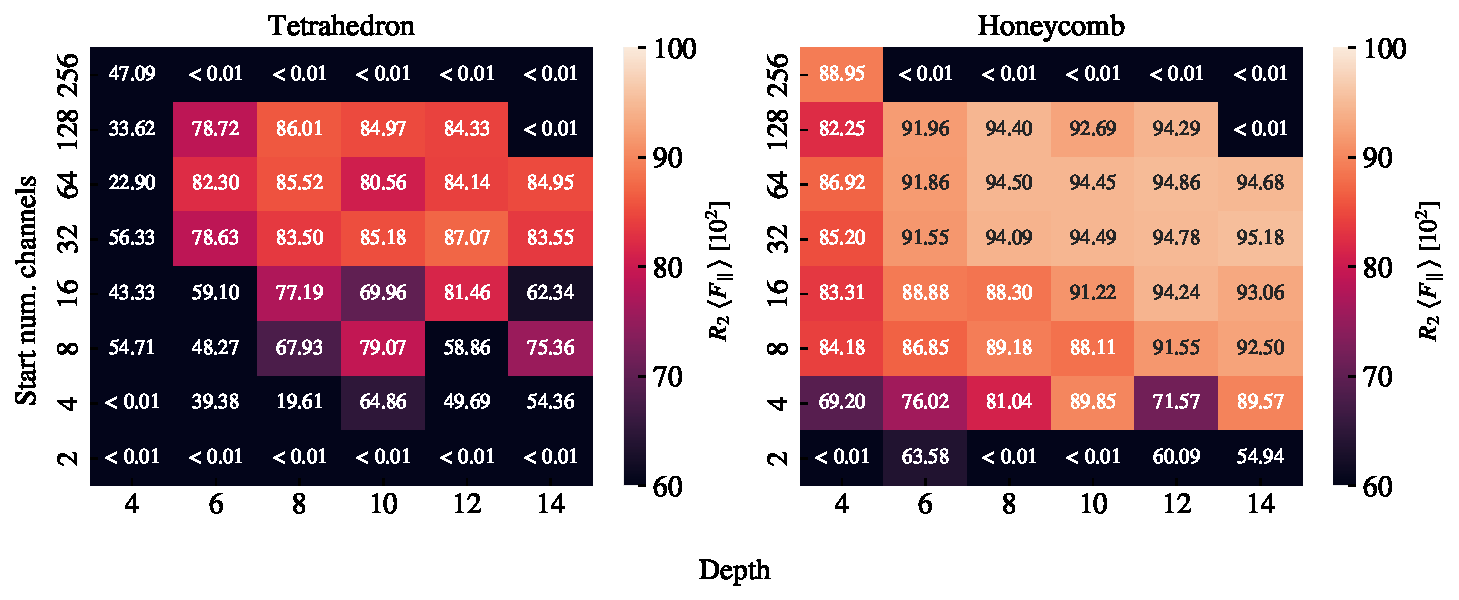
\includegraphics[width=\linewidth]{figures/ML/A_search_compare_perf}
  \caption{Selected pseudo validation set. \hl{Fix the missing grey fields in the top which are replaced by < 0.01.}}
  \label{fig:A_search_compare}
\end{figure}  

From the validation scores in \cref{fig:A_search_perf} we find that models
S(8-32)D(8-12) to give the best performance. When looking at the best epoch we
find that models of low depth result in a later best epoch which is compatible
with underfitting. As the depth is increased we find more models with a lower
best epoch, in the range $\sim [300, 600]$, which on the other hand suggest
cases of overfitting. Since our training stores the best model during training,
we do not have to worry too much about overfitting, but we can take this
transition from underfitting to overfitting as a sign that our search is
conducted in an appropriate complexity range. When consulting the evaluation on the
selected set in \cref{fig:A_search_compare} we notice in general that we get
significantly lower $R_2$ scores, especially for the Tetrahedron pattern. Considering, that some of these data points are also present in the training data, this is a clear indication that these configurations are more challeging to predict. While the peak $R_2$ value for the validation score was found for the S16D10 model we see a slight preference for more complexity in the model with regard to the selected test. In the Tetrahedron selected set grid search, we find the best model to be S32D12, with a $R_2$ score of $\sim 87 \%$. This model choice is more or less compatible with the overall performance as this is among the top candidates for the $R_2$ score and loss in \cref{fig:A_search_perf} and the $R_2$ score for the Honeycomb pattern in \cref{fig:A_search_compare} as well. Hence, we settle on this architecture.


Next, we consider momentum $m$ and weight decays $wd$ in the range $m \in [0.85,
0.99]$ and $wd \in [0, 1e-2]$. An increased momentum is expected to decrease the
appropriate learning rate \hl{(check with theory)}, and thus we perform a new learning rate range test
for each momentum choice. We propose two learning rate schemes: A constant
learning rate as used until this point and a one-cycle policy. In the one-cycle
policy we set a maximum bound for the learning rate and start from a factor
$1/20$ of this bound and increase towards the maximum bound during the first
30\% of the training. For the final 70\% of training we decrease towards a final
minimum given as a factor $1e-4$ of the maximum bound . The increase and
decrease are done by a cosine function. The suggested learning rate for the
constant learning rate scheme is once again determined by the steepest slope on
the loss curve while the maximum bound used for the one-cycle policy is
determined as the point just before divergence. We find that the minimum point
on the loss curve is a suitable choice that approaches the diverging point
without getting too close and causing instabilities. The learning rate range
test for momentum is shown in \cref{fig:LR_range_mom}. \hl{We observe that a higher momentum giver higher suggested learning rates, so I need to check with theory on that}. Using the results for the momentum learning rate range test we perform a grid search of momentum and
weight decay. We examine again the validation loss and validation mean friction
$R_2$ score in addition to the friction mean $R_2$ score for the selected set of
Tetrahedron and Honeycomb patterns. This is shown for the constant learning rate
scheme in \cref{fig:mom_weight_search_constant} and for the cyclic scheme in
\cref{fig:mom_weight_search_cyclic}.

\begin{figure}[H]
  \centering
  \begin{subfigure}[t]{0.49\textwidth}
      \centering
      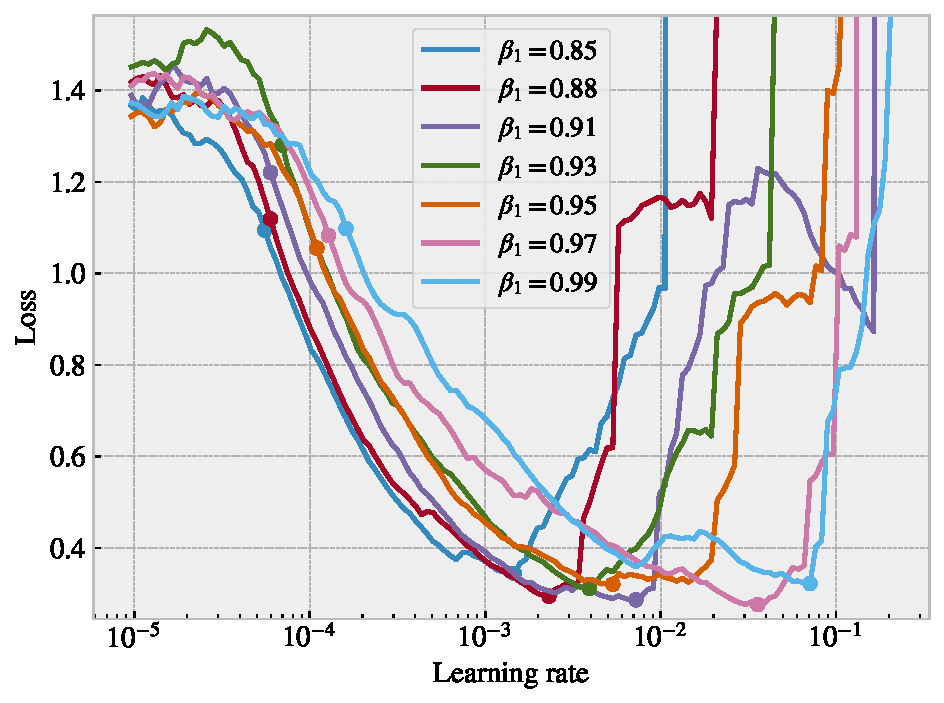
\includegraphics[width=\textwidth]{figures/ML/LR_momentum_test_a.pdf}
      \caption{}
      % \label{fig:}
  \end{subfigure}
  \hfill
  \begin{subfigure}[t]{0.49\textwidth}
      \centering
      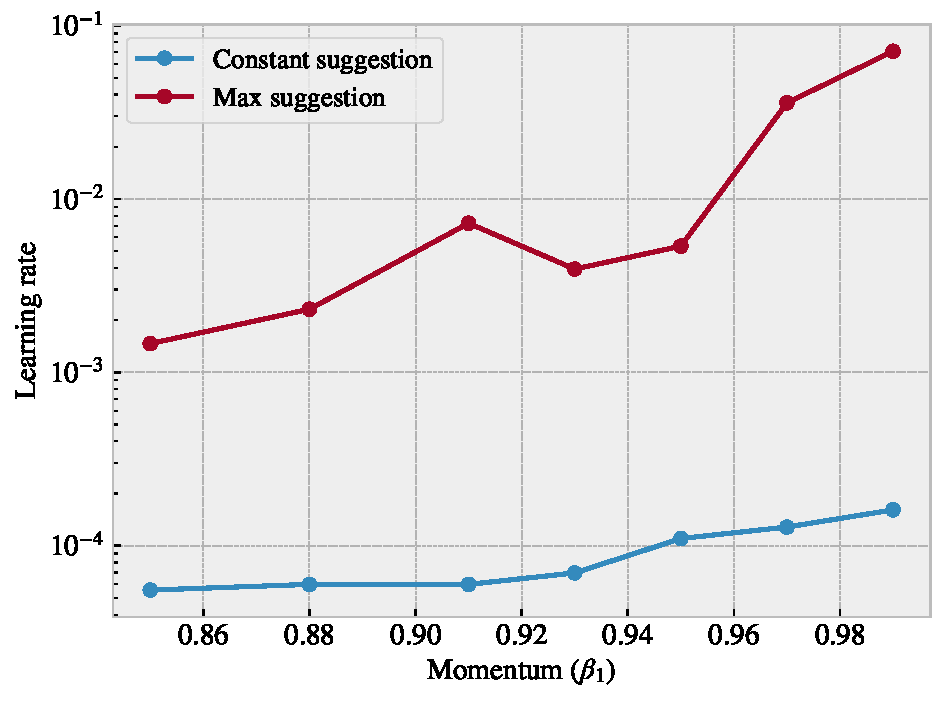
\includegraphics[width=\textwidth]{figures/ML/LR_momentum_test_b.pdf}
      \caption{}
      % \label{fig:}
  \end{subfigure}
  \hfill
  \caption{Momentum learning rate range tets}
  \label{fig:LR_range_mom}
\end{figure}


\begin{figure}[H]
  \centering
  \begin{subfigure}[t]{1.0\textwidth}
      \centering
      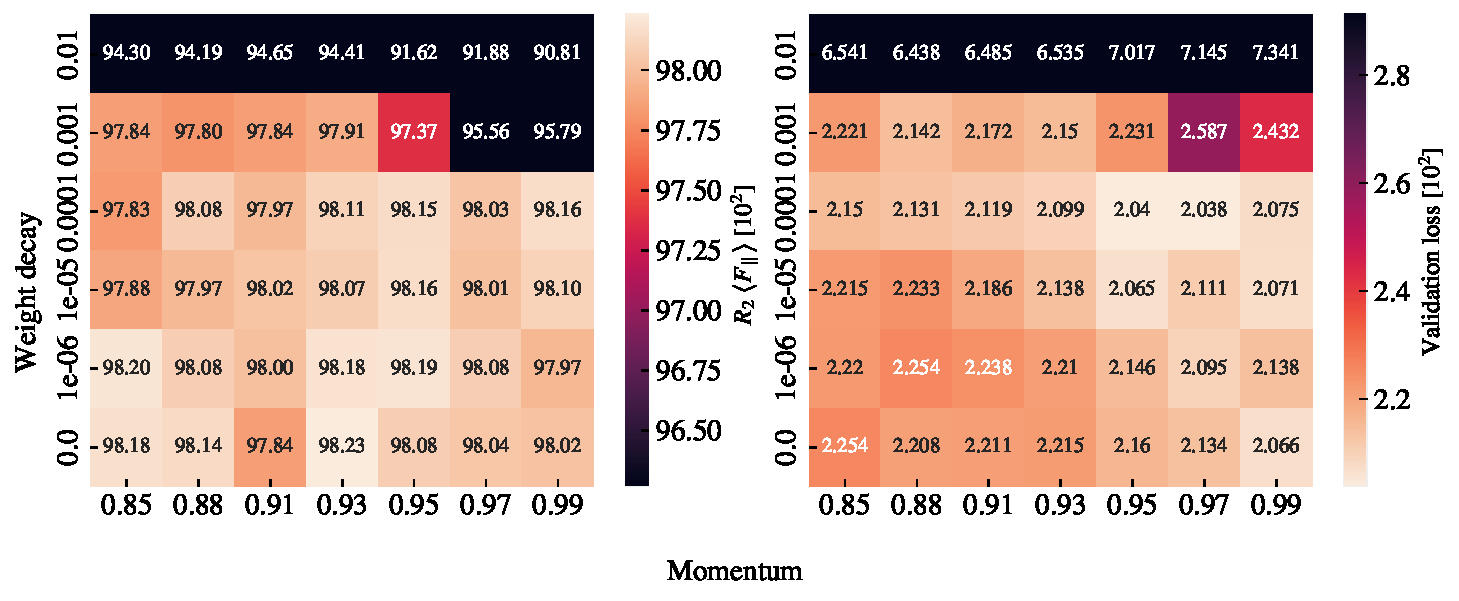
\includegraphics[width=\textwidth]{figures/ML/mom_weight_search_constant_perf.pdf}
      \caption{Validation performance.}
      % \label{fig:}
  \end{subfigure}
  \hfill
  \begin{subfigure}[t]{1.0\textwidth}
      \centering
      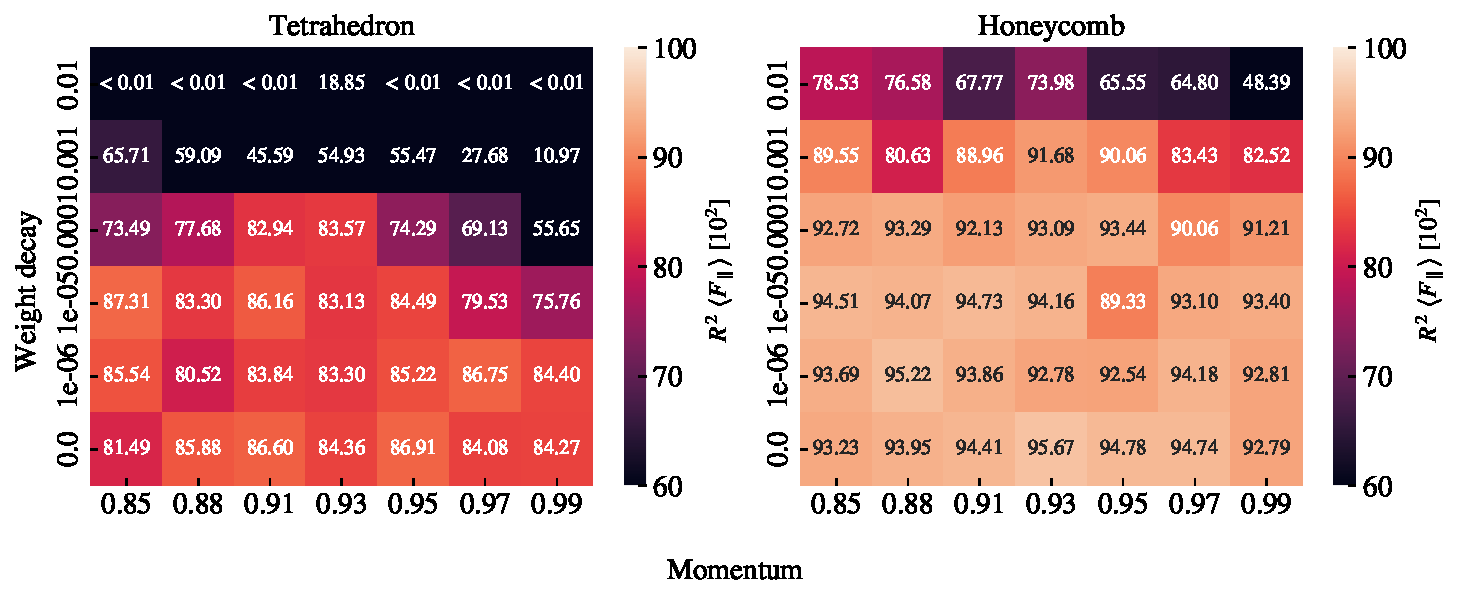
\includegraphics[width=\textwidth]{figures/ML/mom_weight_search_compare_constant_perf.pdf}
      \caption{Selected set comparison.}
      % \label{fig:}
  \end{subfigure}
  \hfill
  \caption{Constant learning rate and momentum scheme}
  \label{fig:mom_weight_search_constant}
\end{figure}

\begin{figure}[H]
  \centering
  \begin{subfigure}[t]{1.0\textwidth}
      \centering
      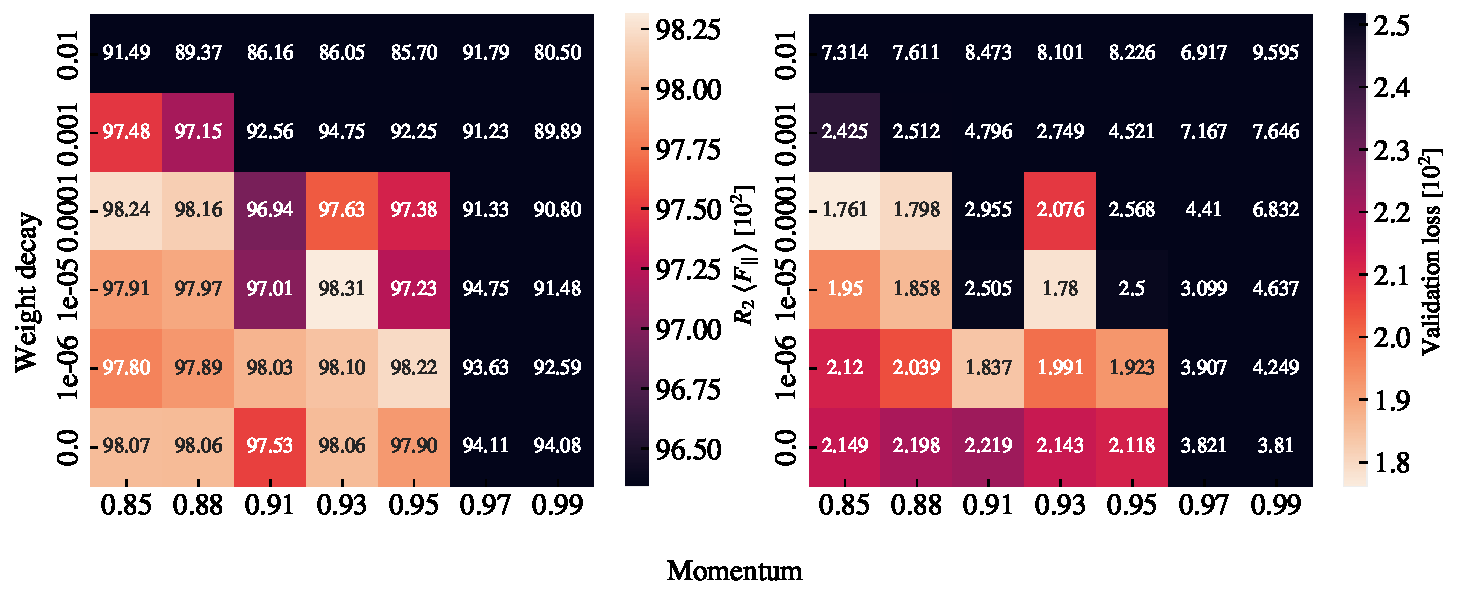
\includegraphics[width=\textwidth]{figures/ML/mom_weight_search_cyclic_perf.pdf}
      \caption{Validation performance.}
      % \label{fig:}
  \end{subfigure}
  \hfill
  \begin{subfigure}[t]{1.0\textwidth}
      \centering
      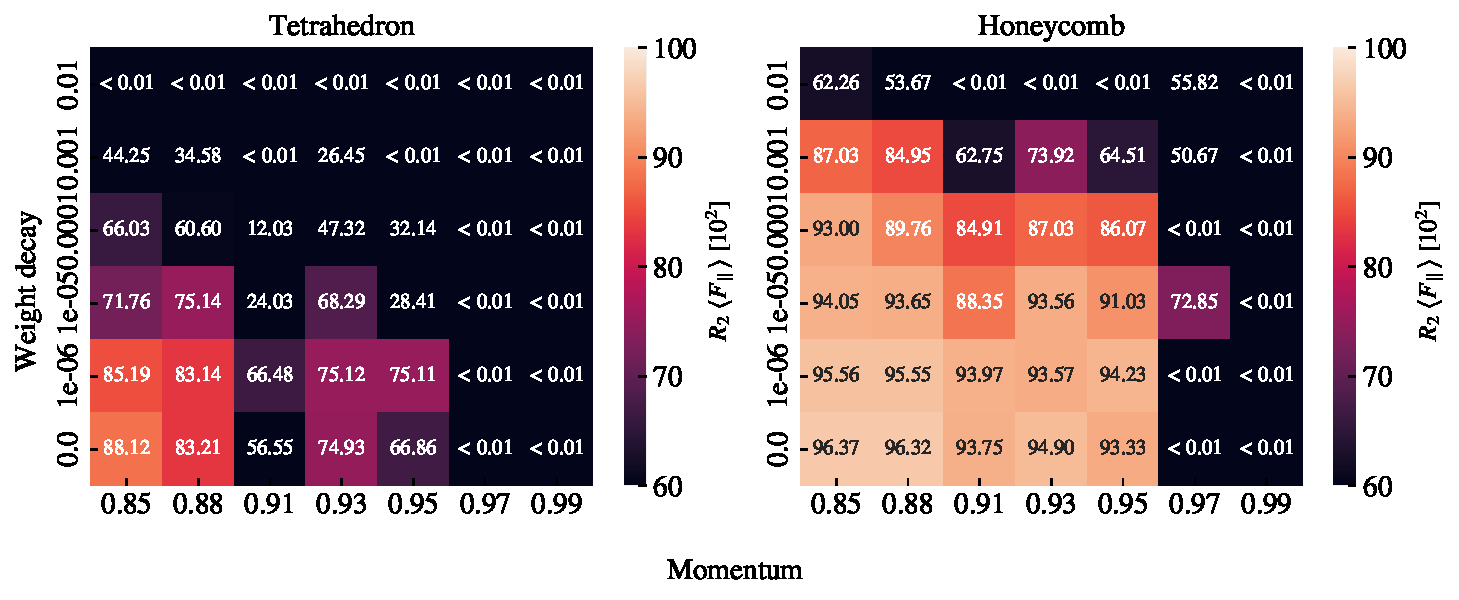
\includegraphics[width=\textwidth]{figures/ML/mom_weight_search_compare_cyclic_perf.pdf}
      \caption{Selected set comparison.}
      % \label{fig:}
  \end{subfigure}
  \hfill
  \caption{Cyclic learning rate and momentum scheme}
  \label{fig:mom_weight_search_cyclic}
\end{figure}


The original validation scores, before varying momentum and weight decay, were a
validation loss of 0.02124 and a mean friction $R_2$ score of 0.9816. By varying
momentum and weight decay, we can improve these scores slightly for the constant
learning rate scheme (loss: 0.02038, $R_2$: 0.9823) and even more for the cyclic
scheme (loss: 0.0176, $R_2$: 0.9831). However, notice that these scores a taking
for separate combinations of hyperparameters. The comparison among best scores is
summarized in \cref{tab:mom_weight_search}. In general, the constant scheme
shows rather stable results for all momentum settings $m \in [0.85, 0.99]$ in
combination with a low weight decay $wd \le \num{e-4}$. For the cyclic scheme
the performance peaks towards a low momentum $m \le 0.93$ and low weight decay
$wd \le \num{e-4}$. Looking at the summary in \cref{tab:mom_weight_search} we
see that the cyclic scheme can produce a high score among all four
performance metrics, but since these scores do not share common hyperparameters we need to choose which of them to prioritize. Due to our interest in capturing the non-linear trends, we prioritize the score from the
selected set of Tetrahedron patterns as this provided the greatest challenge for our model to capture. We recognize that this choice introduces a greater risk of
overfitting since the data points are partly included in the training set. However, for the purpose of performing an accelerated search, we find it more important to increase the chances of discovering novel designs than to reduce the chance of getting false positive results. Since we have the option to verify the properties of a given design through \acrshort{MD} simulations we do not have to rely on the machine learning prediction as a final score but only as a proposal for configurations worth further studing. Thus we choose the cyclic trained model with low momentum $m = 0.85$ and zero weight decay as our final model. Finally, we note that since our choice of hyperparameters corresponded to the edge of our grid search it would have been natural to perform an extended search in that range. This was omitted due to time prioritization and the belief that the potential gain of doing so was not huge.


\begin{table}[H]
  \begin{center}
  \caption{Momentum and weight decay grid search using S32D12 model.}
  \label{tab:mom_weight_search}
  \begin{tabular}{|c|c|c|c|c|} \hline
     &  & Score [\num{e2}] & Momentum & Weight decay \\ \hline
     \multirow{3}{*}{Validation loss} & Original & 2.124 & 0.9 & 0  \\ 
      & Constant & 2.038 & 0.97 & \num{e-4} \\ 
      & Cyclic & 1.761 & 0.85 & \num{e-4} \\ \hline
     \multirow{3}{*}{Validation $R_2$} & Original & 98.16 & 0.9 & 0  \\ 
      & Constant & 98.23 & 0.93 & 0 \\ 
      & Cyclic & 98.31 & 0.93 & \num{e-5} \\ \hline
     \multirow{3}{*}{Tetrahedron $R_2$} & Original & 87.07 & 0.9 & 0  \\ 
      & Constant & 87.31 & 0.85 & \num{e-5} \\ 
      & Cyclic & 88.12 & 0.85 & 0 \\ \hline
     \multirow{3}{*}{Honeycomb $R_2$} & Original & 94.78 & 0.9 & 0  \\ 
      & Constant & 95.67 & 0.93 & 0 \\ 
      & Cyclic & 96.37 & 0.85 & 0 \\ \hline
  \end{tabular}
  \end{center}
\end{table}


% Look at training history plots an show the overfitting (after best epoch)




\subsection{Final model}
From the hypertuning study, we choose the S32D12 model trained by a cyclic
training scheme with a momentum of 0.85 and zero weight decay. The main
performance metrics are shown in \cref{tab:final_model_eval}. Since the porosity
is a number between $0$ and $1$ we can interpret the absolute error as the
percentage error similar to the relative error for the rupture stretch. The
rupture stretch is generally within a 13 \% margin, but we believe that this
number is especially high due to some low stretch rupture cases in the dataset
which contributes to a large relative error. The stretch curves for mean
friction, max friction and contact is shown in \cref{fig:final_model_eval} in
comparison with the Tetrahedron (7, 5, 1) and Honeycomb (2,2,1,5) used in the
pilot study. This gives a visual interpretation of how well the fits are for the
given $R_2$, and we get a visual confirmation that a $R_2$ score above 0.98
indeed looks like a promising capture for the non-linear trends in the data. We will perform a true test set evaluation later on, based on some of the suggestions from the accelerated search.

\begin{table}[H]
  \begin{center}
  \caption{Mean values are used over different configurations.}
  \label{tab:final_model_eval}
  \begin{tabular}{ | c | c | c | c | c | c | c | c |} \hline
    & Loss [\num{e2}] & \multicolumn{3}{c|}{$R_2$ [\num{e2}]} & Abs. [\num{e2}] & Rel. [\num{e2}]  & Acc. [\num{e2}] \\ \hline
    & Total & Mean $F_f$ & Max $F_f$ & Contact & Porosity & Rup.\ Stretch & Rupture \\ \hline
  Validation  & 2.1488 & 98.067 & 93.558 & 94.598 & 02.325 & 12.958 & 96.102 \\ \hline
  Tetrahedron & 4.0328 & 88.662 & 85.836 & 64.683 & 01.207 & 05.880 & 99.762 \\ \hline
  Honeycomb   & 8.6867 & 96.627 & 89.696 & 97.171 & 01.040 & 01.483 & 99.111 \\ \hline
  \end{tabular}
  \end{center}
\end{table}


\begin{figure}[H]
  \centering
  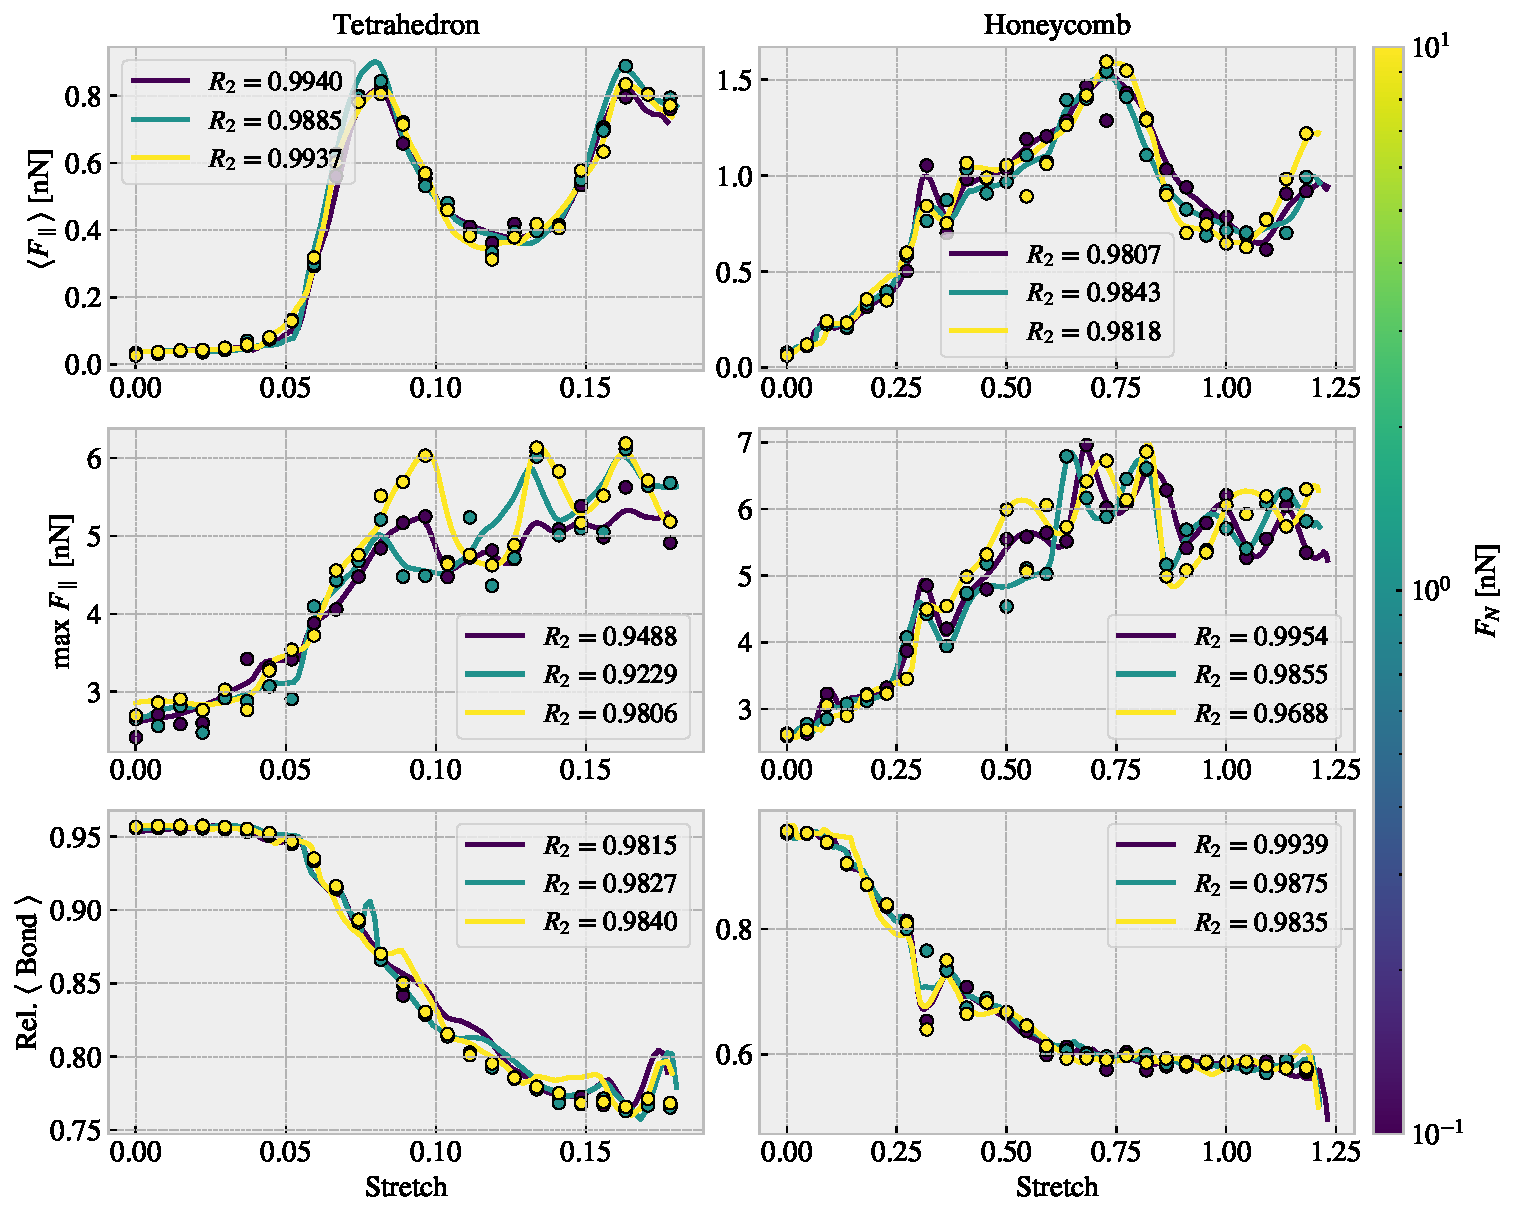
\includegraphics[width=\linewidth]{figures/ML/final_model_evaluation.pdf}
  \caption{With \num{e3} points in the stretch range [0, 1.5] and stopping after first rupture True prediction.}
  \label{fig:final_model_eval}
\end{figure}  

Using our final model, we evaluate the performance for the top ranking within
the properties of interest. That is, we go through all the configurations in the
dataset for the Tetrahedron (\cref{tab:ML_ranking_pop}), Honeycomb
(\cref{tab:ML_ranking_hon}) and Random Walk (\cref{tab:ML_ranking_RW}) patterns
separately and rank the configurations in each property category. This is then compared to the actual ranking in the dataset. Generally, we find that the \acrshort{ML} performs rather well in the ranking of the max, max difference and max drop properies, but it is deviating a bit more for the minimum friction property. This can be attritbuted to the fact that the precision needed for an accurate ranking among the minimum friction cases is a lot greater than for the remaining properties. The \acrshort{ML} model gives mostly similar predictions for the max-categories ranking for the Tetrahedron and Honeycomb pattern but struggles a bit more for the Random Walk. Looking at the values for the top candidates in the max-types properties we see that it is generally within a $\sim 0.2$ nN range which is promising. 

\begin{table}[H]
  \begin{center}
  \caption{Tetrahedon}
  \label{tab:ML_ranking_pop}
  \begin{tabular}{|c|c|c?{0.3mm}c|c|c|} \hline
    ML & \multicolumn{2}{c?{0.3mm}}{Data} &  \multicolumn{2}{c|}{\acrshort{ML}} & Data \\ \cline{2-5}
    Rank & Config & Value [nN] & Config & Value [nN] & Rank \\ \hline
    \multicolumn{6}{|c|}{$\min F_{\text{fric}}$} \\ \hline
    20 & (3, 9, 4) & 0.0067 & (3, 1, 2) & 0.0041 & 5  \\ \hline
    5 & (3, 1, 3) & 0.0075 & (1, 3, 4) & 0.0049 & 11 \\ \hline
    6 & (5, 3, 4) & 0.0084 & (1, 3, 3) & 0.0066 & 6  \\ \hline
    21 & (1, 7, 3) & 0.0084 & (3, 1, 4) & 0.0066 & 8  \\ \hline
    1 & (3, 1, 2) & 0.0097 & (3, 1, 3) & 0.0078 & 2  \\ \hline
    \multicolumn{6}{|c|}{$\max F_{\text{fric}}$} \\ \hline
    1 & (5, 3, 1) & 1.5875 & (5, 3, 1) & 1.5920 & 1 \\ \hline
    2 & (1, 3, 1) & 1.4310 & (1, 3, 1) & 1.2739 & 2 \\ \hline
    4 & (3, 1, 2) & 1.0988 & (9, 3, 1) & 1.1162 & 4 \\ \hline
    3 & (9, 3, 1) & 1.0936 & (3, 1, 2) & 0.7819 & 3 \\ \hline
    5 & (7, 5, 1) & 0.7916 & (7, 5, 1) & 0.7740 & 5 \\ \hline
    \multicolumn{6}{|c|}{$\max \Delta F_{\text{fric}}$} \\ \hline
    1 & (5, 3, 1) & 1.5529 & (5, 3, 1) & 1.5578 & 1 \\ \hline 
    2 & (1, 3, 1) & 1.3916 & (1, 3, 1) & 1.2331 & 2 \\ \hline 
    4 & (3, 1, 2) & 1.0891 & (9, 3, 1) & 1.0807 & 4 \\ \hline 
    3 & (9, 3, 1) & 1.0606 & (3, 1, 2) & 0.7778 & 3 \\ \hline 
    5 & (7, 5, 1) & 0.7536 & (7, 5, 1) & 0.7399 & 5 \\ \hline 
    \multicolumn{6}{|c|}{max drop} \\ \hline
    1 & (5, 3, 1) & 0.8841 & (5, 3, 1) & 0.8603 & 1 \\ \hline 
    2 & (3, 5, 1) & 0.4091 & (3, 5, 1) & 0.3722 & 2 \\ \hline 
    4 & (7, 5, 1) & 0.3775 & (1, 1, 1) & 0.2879 & 5 \\ \hline 
    5 & (9, 7, 1) & 0.2238 & (7, 5, 1) & 0.2478 & 3 \\ \hline 
    3 & (1, 1, 1) & 0.1347 & (9, 7, 1) & 0.1302 & 4 \\ \hline 
  \end{tabular}
  \end{center}
\end{table}

\begin{table}[H]
  \begin{center}
  \caption{Honeycomb}
  \label{tab:ML_ranking_hon}
  \begin{tabular}{|c|c|c?{0.3mm}c|c|c|} \hline
    ML & \multicolumn{2}{c?{0.3mm}}{Data} &  \multicolumn{2}{c|}{\acrshort{ML}} & Data \\ \cline{2-5}
    Rank & Config & Value [nN] & Config & Value [nN] & Rank \\ \hline
    \multicolumn{6}{|c|}{$\min F_{\text{fric}}$} \\ \hline
    1 & (2, 5, 1, 1) & 0.0177 & (2, 5, 1, 1) & 0.0113 & 1 \\ \hline 
    9 & (2, 4, 5, 1) & 0.0187 & (2, 5, 5, 3) & 0.0149 & 7 \\ \hline 
    7 & (2, 4, 1, 1) & 0.0212 & (2, 5, 5, 1) & 0.0182 & 4 \\ \hline 
    3 & (2, 5, 5, 1) & 0.0212 & (2, 5, 3, 1) & 0.0186 & 5 \\ \hline 
    4 & (2, 5, 3, 1) & 0.0226 & (2, 4, 1, 3) & 0.0198  & 15 \\ \hline 
    \multicolumn{6}{|c|}{$\max F_{\text{fric}}$} \\ \hline
    1 & (2, 1, 1, 1) & 2.8903 & (2, 1, 1, 1) & 2.9171 & 1 \\ \hline 
    2 & (2, 1, 5, 3) & 2.2824 & (2, 1, 5, 3) & 2.4004 & 2 \\ \hline 
    6 & (2, 1, 3, 1) & 2.0818 & (2, 1, 5, 1) & 2.1060 & 5 \\ \hline 
    4 & (2, 1, 3, 3) & 2.0313 & (2, 1, 3, 3) & 1.9458 & 4 \\ \hline 
    3 & (2, 1, 5, 1) & 2.0164 & (2, 4, 1, 1) & 1.9381 & 6 \\ \hline 
    \multicolumn{6}{|c|}{$\max \Delta F_{\text{fric}}$} \\ \hline
    1 & (2, 1, 5, 3) & 2.0234 & (2, 1, 5, 3) & 2.1675 & 1 \\ \hline 
    2 & (2, 1, 1, 1) & 1.9528 & (2, 1, 1, 1) & 2.0809 & 2 \\ \hline 
    3 & (2, 4, 1, 1) & 1.8184 & (2, 4, 1, 1) & 1.9157 & 3 \\ \hline 
    4 & (2, 1, 3, 3) & 1.7645 & (2, 1, 3, 3) & 1.6968 & 4 \\ \hline 
    5 & (2, 4, 1, 3) & 1.4614 & (2, 4, 1, 3) & 1.5612 & 5 \\ \hline 
    \multicolumn{6}{|c|}{max drop} \\ \hline
    1 & (2, 3, 3, 3) & 1.2785 & (2, 3, 3, 3) & 1.3642 & 1 \\ \hline 
    2 & (2, 1, 3, 1) & 1.1046 & (2, 1, 3, 1) & 0.9837 & 2 \\ \hline 
    3 & (2, 3, 3, 5) & 0.8947 & (2, 3, 3, 5) & 0.9803 & 3 \\ \hline 
    4 & (2, 1, 5, 3) & 0.8638 & (2, 1, 5, 3) & 0.9556 & 4 \\ \hline 
    13 & (2, 5, 1, 1) & 0.8468 & (2, 4, 5, 3) & 0.8999 & 8 \\ \hline 
  \end{tabular}
  \end{center}
\end{table}


\begin{table}[H]
  \begin{center}
  \caption{RW}
  \label{tab:ML_ranking_RW}
  \begin{tabular}{|c|c|c?{0.3mm}c|c|c|} \hline
    ML & \multicolumn{2}{c?{0.3mm}}{Data} &  \multicolumn{2}{c|}{\acrshort{ML}} & Data \\ \cline{2-5}
    Rank & Config & Value [nN] & Config & Value [nN] & Rank \\ \hline
    \multicolumn{6}{|c|}{$\min F_{\text{fric}}$} \\ \hline
    1 & 12 & 0.0024 & 12 & -0.0011 & 1 \\ \hline 
    24 & 76 & 0.0040 & 06 & 0.0036  & 27 \\ \hline 
    6 & 13 & 0.0055 & 14 & 0.0074  & 23 \\ \hline 
    31 & 08 & 0.0065 & 05 & 0.0082  & 19 \\ \hline 
    26 & 07 & 0.0069 & 63 & 0.0085  & 57 \\ \hline 
    \multicolumn{6}{|c|}{$\max F_{\text{fric}}$} \\ \hline
    3 & 96 & 0.5758 & 99 & 0.5155 & 2 \\ \hline 
    1 & 99 & 0.5316 & 98 & 0.4708 & 3 \\ \hline 
    2 & 98 & 0.4478 & 96 & 0.4356 & 1 \\ \hline 
    4 & 97 & 0.3624 & 97 & 0.3503 & 4 \\ \hline 
    11 & 58 & 0.3410 & 55 & 0.2817 & 7 \\ \hline 
    \multicolumn{6}{|c|}{$\max \Delta F_{\text{fric}}$} \\ \hline
    3 & 96 & 0.5448 & 99 & 0.4669 & 2 \\ \hline 
    1 & 99 & 0.4769 & 98 & 0.4314 & 3 \\ \hline 
    2 & 98 & 0.4085 & 96 & 0.4128 & 1 \\ \hline 
    4 & 97 & 0.3268 & 97 & 0.3080 & 4 \\ \hline 
    78 & 57 & 0.2978 & 55 & 0.2542 & 7 \\ \hline 
    \multicolumn{6}{|c|}{max drop} \\ \hline
    3 & 01 & 0.1818 & 00 & 0.1883 & 3 \\ \hline 
    2 & 96 & 0.1733 & 96 & 0.1654 & 2 \\ \hline 
    1 & 00 & 0.1590 & 01 & 0.1532 & 1 \\ \hline 
    11 & 37 & 0.1022 & 04 & 0.0591 & 8 \\ \hline 
    28 & 34 & 0.0879 & 56 & 0.0552 & 20 \\ \hline 
  \end{tabular}
  \end{center}
\end{table}


\section{Accelerated Search}

Having trained a machine learning (\acrshort{ML}) model we use it for an extended accelerated search for further optimization of the friction properties of interest. We approach this search by two different methods:
\begin{enumerate}
  \item Using the generative algorithms developed for the creation of the Tetrahedron, Honeycomb and Random walk patterns, we create yet an extended dataset and evaluate the performance using the \acrshort{ML}.
  \item Using the genetic algorithm method we perpetuate the configurations and optimize for the maximum drop property using the \acrshort{ML} model to evaluate the fitness function. 
\end{enumerate}


\subsection{Patteren generation search}
% Judging from the ranking in \cref{tab:ML_ranking_pop}, \cref{tab:ML_ranking_hon} and
% \cref{tab:ML_ranking_RW}, the \acrshort{ML} model showcases a reasonable
% performance with respect to the task of assigning ordinal numbers, i.e.\ predictiong the relative ranking, to the configurations. 

We utilize the pattern generators to create an extended dataset for our search. For the Tetrahedron and Honeycomb patterns, the increment of the parameters will eventually lead to the main structures becoming so large they do exceed the size of the sheet. Thus, we can essentially perform a
full search ``maxing out'' the parameters of these patterns. We estimate
that this is done with the max parameters, $(60, 60, 30)$ for the Tetrahedron,
and $([30, 30, 30, 60])$ for the Honeycomb. We use a random reference position
and regenerate each unique parameter 10 times to explore translational effects. This gives in total 135k configurations for the
Tetrahedron pattern and 2025k for the Honeycomb pattern. For the Random walk
generator, we do a Monte Carlo sampling. In each sample, we draw the scalar values, either from a uniform (U) or logarithmic uniform (LU) distribution as follows.
\begin{align*}
  \text{Num. walks} &\sim \text{U}[1, 30] & \text{Max. steps} &\sim \text{U}[1,30]  & \text{Min. dis.} &\sim \text{U}[0,4] \\
  \text{Bias direction} &\sim \text{U}[0, 2\pi] & \text{Bias. strength} &\sim \text{LU}[0,10]  & p_{\text{stay}} &\sim \text{U}[0,1]  
\end{align*}
Notice that we use discrete distribution for the parameters requiring integers. For the binary parameters \textit{Connection}, \textit{Avoid unvalid},
\textit{RN6} and \textit{Grid start} we simply set the values by a 50--50 chance. The remaining parameters are kept constant at \textit{Periodic: True} and \textit{Centering:False} throughout the search. For the handling of clustering, we implement the repair algorithm such that the sheet is repaired by the least modifications approach rather than retrying the generation several times \hl{Make sure that this is introduced somewhere}. Due to the extra computation time associated with the
random walk and the repair algorithm, we only generate 10k configurations within
this class. For the evaluation of the configurations we use a normal load of \SI{5}{nN} and generate a stretch curve in the domain 0--200 \% using 100 evenly spaced points. Top candidate results for each property are shown in
\cref{tab:pattern_search} including a comparison to the dataset top candidates
originally shown in \cref{tab:data_properties}. The random walk top five candidates are visualized in \cref{fig:RW_search_top5}.

First of all, the search shows a rather consistent result regarding the minimization of friction where the top candidates all share the same feature of being sparsely cut. For the Random walk, we see this visually in\cref{fig:RW_search_top5}, while for the Tetrahedon and Honeycomb patterns, this is evident from the configuration parameters shown in
\cref{tab:pattern_search} where the parameters reveal a high spacing between the
cuts. The porosity of the minimum friction top candidates are all rather low being $1.5\%, 5.6\%, 1.6\%$ for the Tetrahedron, Honeycomb and Random walk respectively. These results point towards the fact that the Kirigami modification does not immediately give rise to any lowering of friction, within the numerical and physical domain defined by our simulation setup. This is in agreement with the initial analysis on the \acrshort{MD} dataset, and it is not surprising that the search did not reveal any ... since the dataset did not contain any suggestion how these can be doe.

%
%
\hl{Working here}
%
%



Note that the full ranking did not strictly favor the least amount of
atoms removed, but considering that the relative error is high for this domain we can not expect this kind of precision. The fact that the top candidates all take
negative values also shows that the model is not reliable in this domain. By
asking for the lowest friction we essentially find the weak spots, sparsely populated points in \hl{vector space},  which can lead to unphysical predictions. This problem should most likely be resolved through an extension of the dataset and perhaps by applying a physical constraint to the
model regarding negative values. 

Among the remaining properties, we find competing values for the Honeycomb and Random walk classes only. When taking a closer look to the ranking for each property it became apparent the predictions are highly sensitive
to the reference position parameters used for the Tetrahedron and Honeycomb
pattern. Since we repeated each parameter 10 times with random reference positions, we initially expected to get a ranking in sets of 10. However, the ranking only shows contiguous appearing sets in the range 1--5. Hence we investigate this sensitivity further by evaluating the scores for a systematic change of the reference position for selected configurations. We generally found the mac drop parameter to give the highest variation and thus we show scores for the max drop top candidates, Tetrahedron $(1,7,1)$, $(5,3,1)$ and Honeycomb $(3,3,5,3)$, $(2,3,3,3)$, in
\cref{fig:ref_search_top_data}. It becomes evident that the predictions vary
drastically with translation of these patterns. The emerging question is then whether this is actually grounded in a physical phenomenon or simply a deficiency in the \acrshort{ML}. Even though the patterns are periodic in the x-y-plane, by the number of center elements represented by the shown squares in \cref{fig:ref_search_top_data}, the translation will determine the specific configuration of the edge. Previous studies of static friction and stick-slip behavior point to the importance of edge effects \hl{look back at theory and
maybe source}, and thus for a sheet where the atoms sitting on the $\pm x$ free sides constitutes about 2.5\% of the inner sheet atom count, it is not unreasonable
that the translation might result in a significantly different outcome. In that case, the search through reference positions highlights that the translation can be key to optimizing for certain properties. However, the results might also indicate that the model is either overfitted or that we simply did not provide enough data to reach a generalization of the complex physical behavior of the system. The sensible way forward to unravel this would be to generate additional
translational variants of the same configurations to investigate for any physical edge dependencies or otherwise strengthen the model. We earmark this suggestion for another study. When considering some of the stretch curves we also find that the prediction of the rupture point makes a crucial impact. As the rupture was often predicted on a descending part of the curve any variation to the rupture point will affect the max drop property quite significantly.





\begin{table}[H]
  \begin{center}
  \caption{Pattern search. The values are in units nN.}
  \label{tab:pattern_search}
  \begin{tabular}{|L{1.75cm} |c|c|c| c |c|c|c|} \cline{2-4} \cline{6-8}
  \multicolumn{1}{c|}{} & \multicolumn{3}{c|}{Search}  && \multicolumn{3}{c|}{Data} \\ \cline{2-4} \cline{6-8}
  \multicolumn{1}{c|}{\textbf{Scores}} & Tetrahedron & Honeycomb & Random walk && Tetrahedron & Honeycomb & Random walk \\ \cline{1-4} \cline{6-8}
  $\min F_{\text{fric}}$         & $-0.062 \ \ $  & $-0.109 \ \ $  & $-0.061 \ \ $ &&   0.0067 & 0.0177 & 0.0024 \\ \cline{1-4} \cline{6-8}
  $\max F_{\text{fric}}$         & $1.089$        & $2.917$        & $0.660$       &&   1.5875 & 2.8903 & 0.5758 \\ \cline{1-4} \cline{6-8}
  $\max \Delta F_{\text{fric}}$  & $1.062$        & $2.081$        & $0.629$       &&   1.5529 & 2.0234 & 0.5448 \\ \cline{1-4} \cline{6-8}   
  max drop                      & $0.277$        & $1.250$        & $0.269$       &&   0.8841 & 1.2785 & 0.1818 \\ \cline{1-4} \cline{6-8}   
  \multicolumn{8}{c|}{} \\ \cline{2-4} \cline{6-8}
  \multicolumn{1}{c|}{\textbf{Configs.}} & Tetrahedron & Honeycomb & Random walk  && Tetrahedron & Honeycomb & Random walk  \\ \cline{1-4} \cline{6-8}
  $\min F_{\text{fric}}$         & $(13,11,14)$ & $(14,25,7,19)$  & No naming &&   $(3,9,4)$ & $(2,5,1,1)$ & 12 \\ \cline{1-4} \cline{6-8}
  $\max F_{\text{fric}}$         & $(1,3,1)$    & $(2,1,1,1)$     & No naming &&   $(5,3,1)$ & $(2,1,1,1)$ & 96 \\ \cline{1-4} \cline{6-8}
  $\max \Delta F_{\text{fric}}$  & $(1,3,1)$    & $(2,1,1,1)$     & No naming &&   $(5,3,1)$ & $(2,1,5,3)$ & 96 \\ \cline{1-4} \cline{6-8}   
  max drop                      & $(1,7,1)$    & $(3,3,5,3)$     & No naming &&   $(5,3,1)$ & $(2,3,3,3)$ & 01 \\ \cline{1-4} \cline{6-8}   
  \end{tabular}
  \end{center}
\end{table}


\begin{figure}[H]
  \centering
  \begin{subfigure}[t]{0.49\textwidth}
      \centering
      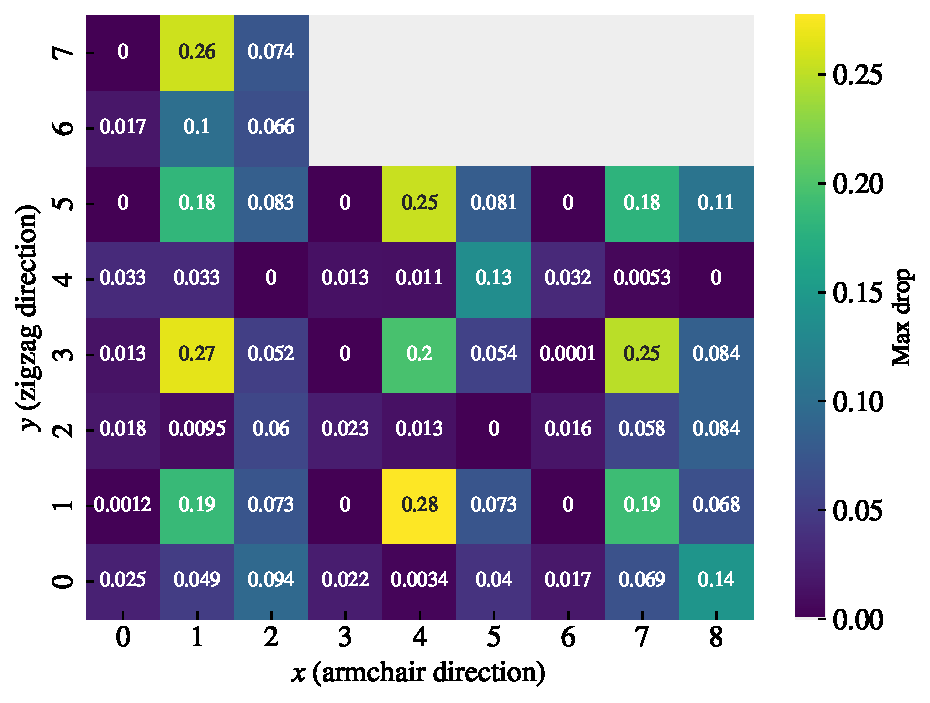
\includegraphics[width=\textwidth]{figures/search/ref_search_drop_pop_1_7_1_ref_search.pdf}
      \caption{Tetrahedron $(1,7,1)$ (60). Std = 0.08, Rel.\ Std = 1.13}
      % \label{fig:}
  \end{subfigure}
  \hfill
  \begin{subfigure}[t]{0.49\textwidth}
    \centering
    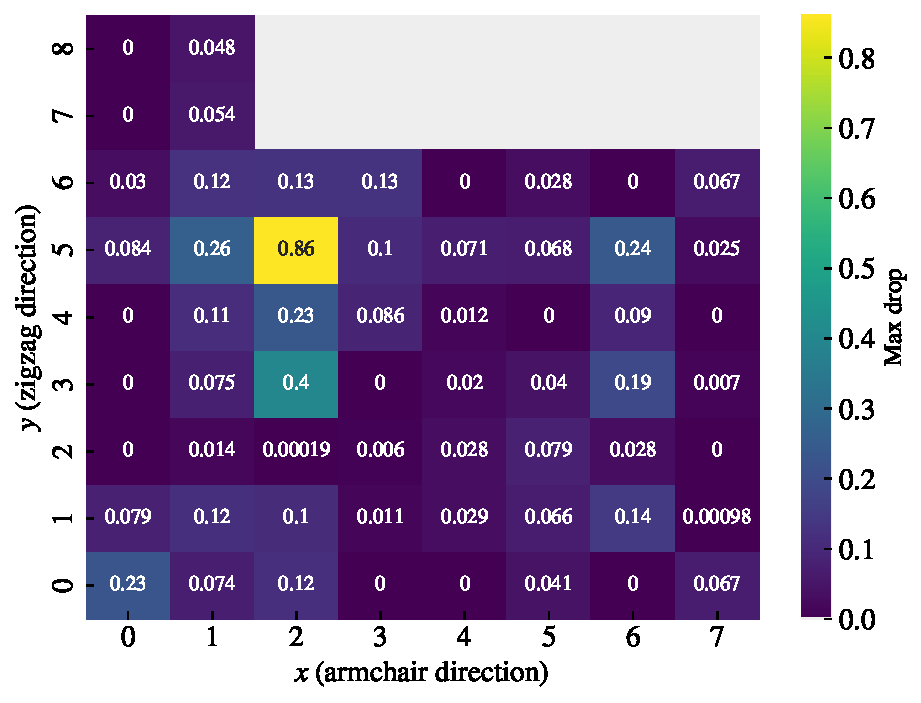
\includegraphics[width=\textwidth]{figures/search/ref_search_drop_pop_5_3_1_ref_search.pdf}
    \caption{Tetrahedron $(5,3,1)$ (60). Std = 0.13, Rel.\ Std = 1.61}
    % \label{fig:}
  \end{subfigure}
  \hfill
  \begin{subfigure}[t]{0.49\textwidth}
      \centering
      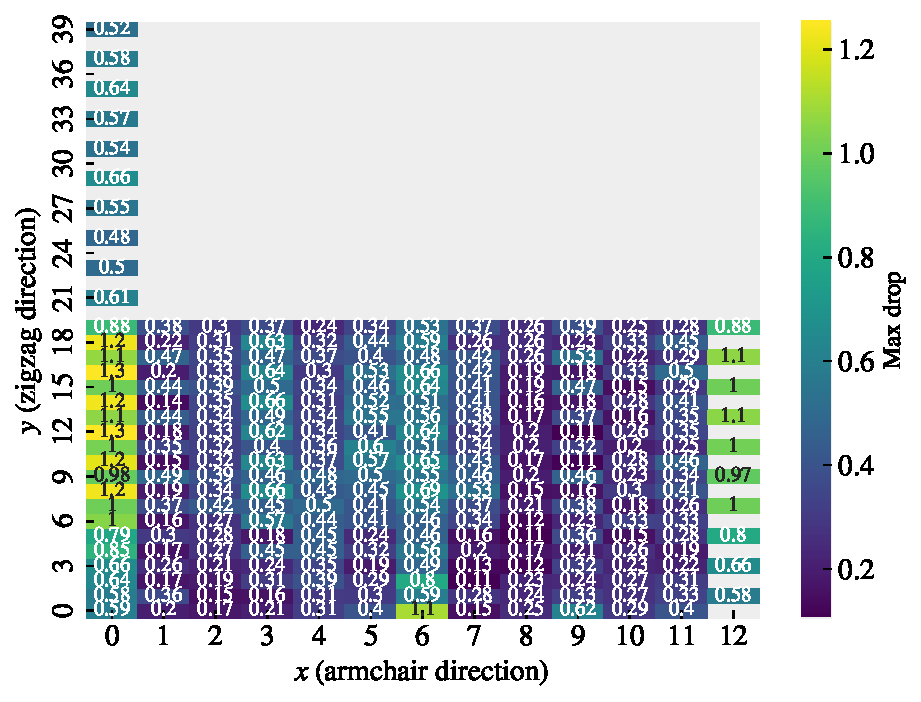
\includegraphics[width=\textwidth]{figures/search/ref_search_drop_hon_3_3_5_3_ref_search.pdf}
      \caption{Honeycomb $(3,3,5,3)$ (260). Std = 0.25, Rel.\ Std = 0.58}
      % \label{fig:}
  \end{subfigure}
  \hfill
  \begin{subfigure}[t]{0.49\textwidth}
      \centering
      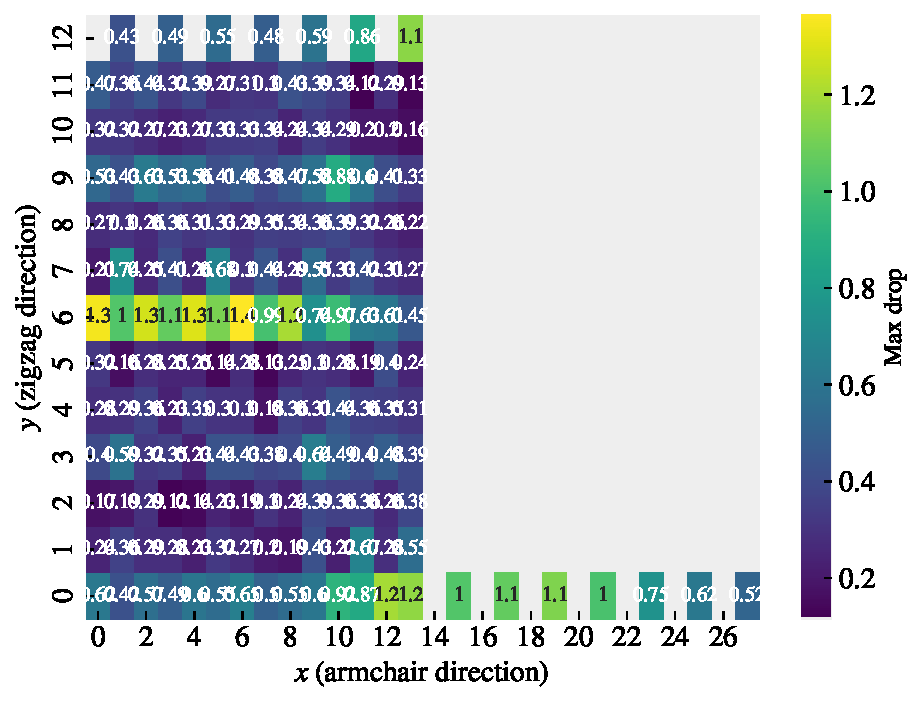
\includegraphics[width=\textwidth]{figures/search/ref_search_drop_hon_2_3_3_3_ref_search.pdf}
      \caption{Honeycomb $(2,3,3,3)$. (182)  Std = 0.27, Rel.\ Std = 0.60}
      % \label{fig:}
  \end{subfigure}
  \hfill
  \caption{\hl{CAPTION}}
  \label{fig:ref_search_top_data}
\end{figure}



\begin{figure}[H]
  \centering
  \includegraphics[width=\linewidth]{figures/search/RW_search_top5.pdf}
  \caption{RW search top results.}
  \label{fig:RW_search_top5}
\end{figure}  



\subsection{Genetic algorithm search}
The second approach to an accelerated search is through the genetic algorithm.
So far we have concluded that a minimization of the friction, with our system
specifications and model predictions, is not promising. Hence, we discard this
property for further study. We have also seen that the maximum style property
often shares similar top candidates, and thus we choose to only investigate the
max drop property, associated with the aim of creating a negative friction
coefficient. From the extended search, we have three candidates within the
Tetrahedron, Honeycomb and Random walk style. We use these three candidates as
the basis for an genetic agorithm search. We generate a population of 100
configurations using the settings associated with the top candidates. We run the
search for 50 generations as we did not see much difference for any longer
extensions. The Tetrahedron and Honeycomb search did not give any improvements
as the top configuration as the first generations was not improved on even
through the average score was rising. This was more or less the case for the
random walk as well with only a single new candidate giving a score of
\SI{0.300}{nN} for the drop property. The fact that starting from an existing
design did not give any useful results we attempted to start from a population
of random noise as well. We did with mixed porosities, even parts of $\{0.01,
0.05, 0.1, 0.2, 0.3\}$, and two for a porosity of 0.25 and 0.5 respectively.
This time the algorithm improved the top candidate throughout, but the actual
scores were disappointing. For the mixed porosity start, we found a top score of
\SI{0.299}{nN}. The top candidates did not seem to carry any higher order
patterns. To the human eye they still looked like random noise. By the use of
the gradient cam method \hl{not sure of name yet} we investigate for any
noticable patterns in the model. This is shown for the mixed porosity top
candidate in \cref{fig:GC_mixed_p} which can be compared to the top search
candidates in the drop category in figure \cref{fig:GC_pop_search}, \cref{fig:GC_hon_search} and \cref{fig:GC_RW_search}. While looking a such gradient visulizations can be mesmerizing they do not immediately reveal more about the underlying mechanisms. The ``attention'' of the model often matches well with the placement of the cuts, but it also reveals some frames where it seems consider the edge quite heavily. This especially relates to to the top and bottom edge which corresponds to the front and back of the sheet. Since these are also connected to the pull block it is really not an edge and thus it is a bit surprising if these should be of extra importance. Given the limited time resources we can follow up on these questions.



\begin{figure}[H]
  \centering
  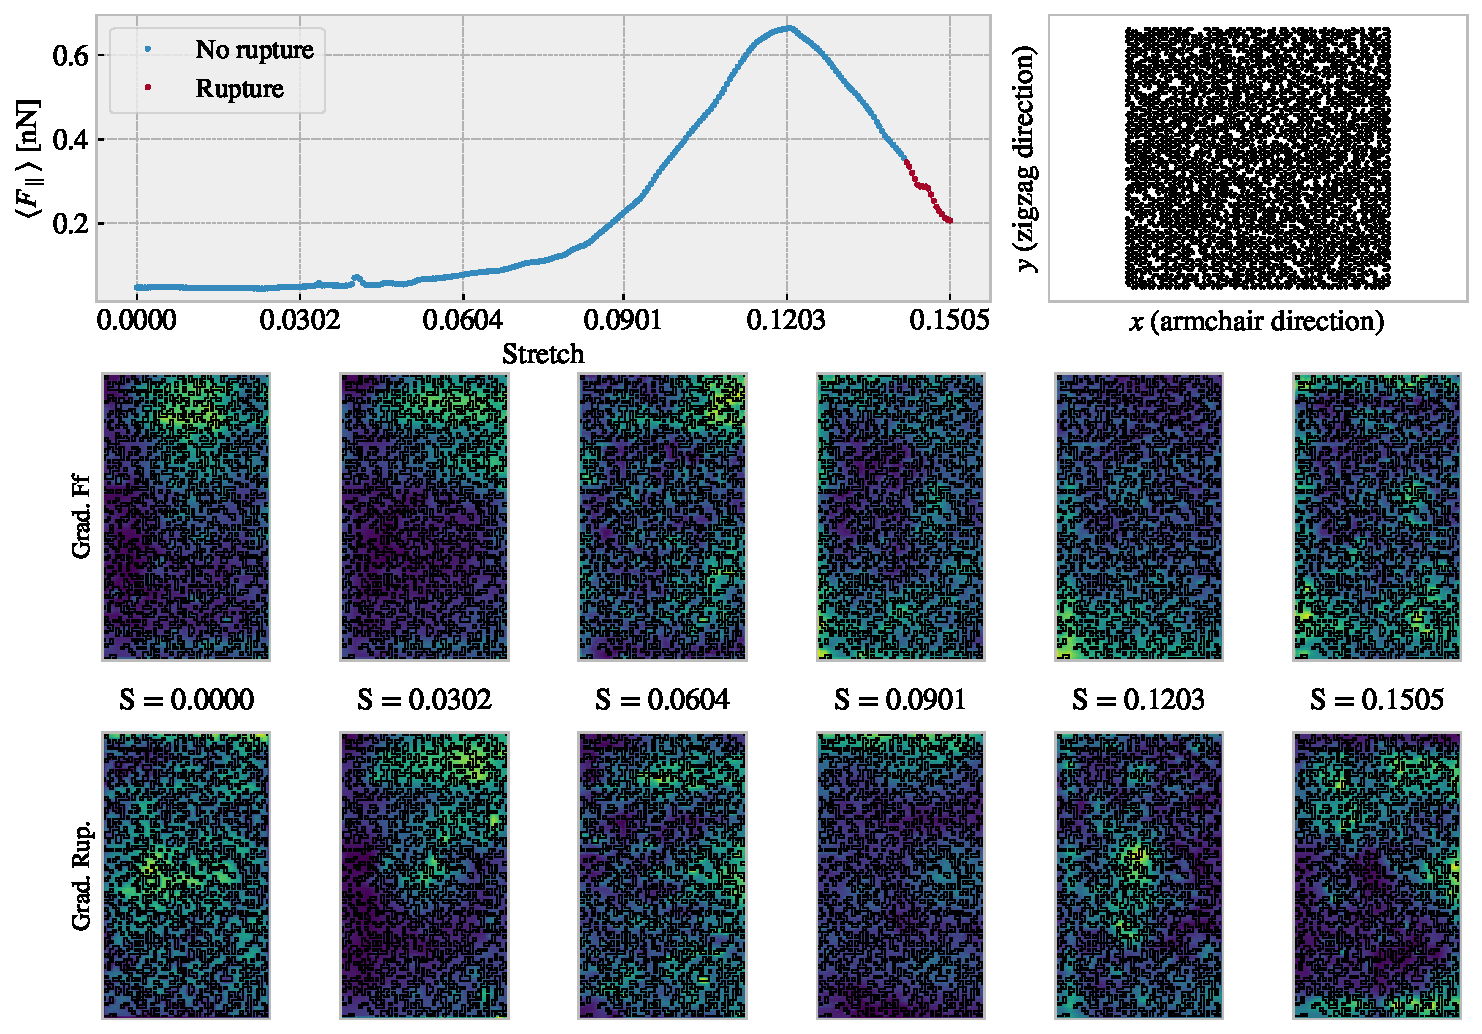
\includegraphics[width=0.8\linewidth]{figures/search/grad_cam_GA_RN_start_top0.pdf}
  \caption{$p \in \{0.01, 0.05, 0.1, 0.2, 0.3\}$.}
  \label{fig:GC_mixed_p}
\end{figure}  

\begin{figure}[H]
  \centering
  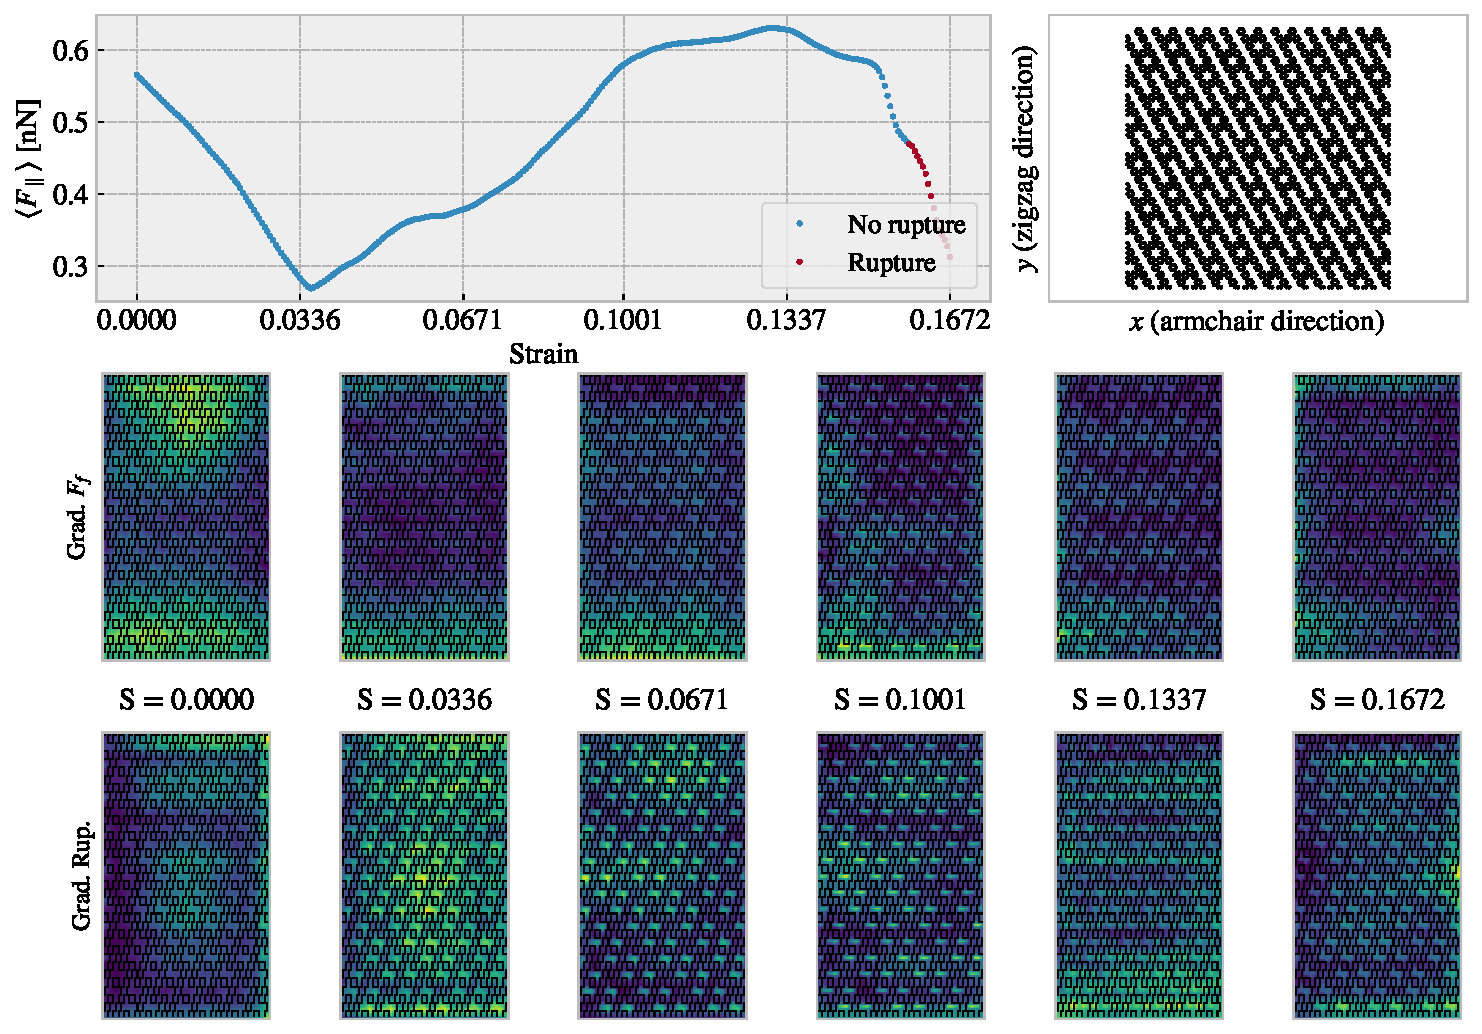
\includegraphics[width=0.8\linewidth]{figures/search/grad_cam_pop_1_7_1_1_4.pdf}
  \caption{Tetrahedron $(1,7,1)$, ref = $(1,4)$}
  \label{fig:GC_pop_search}
\end{figure}  


\begin{figure}[H]
  \centering
  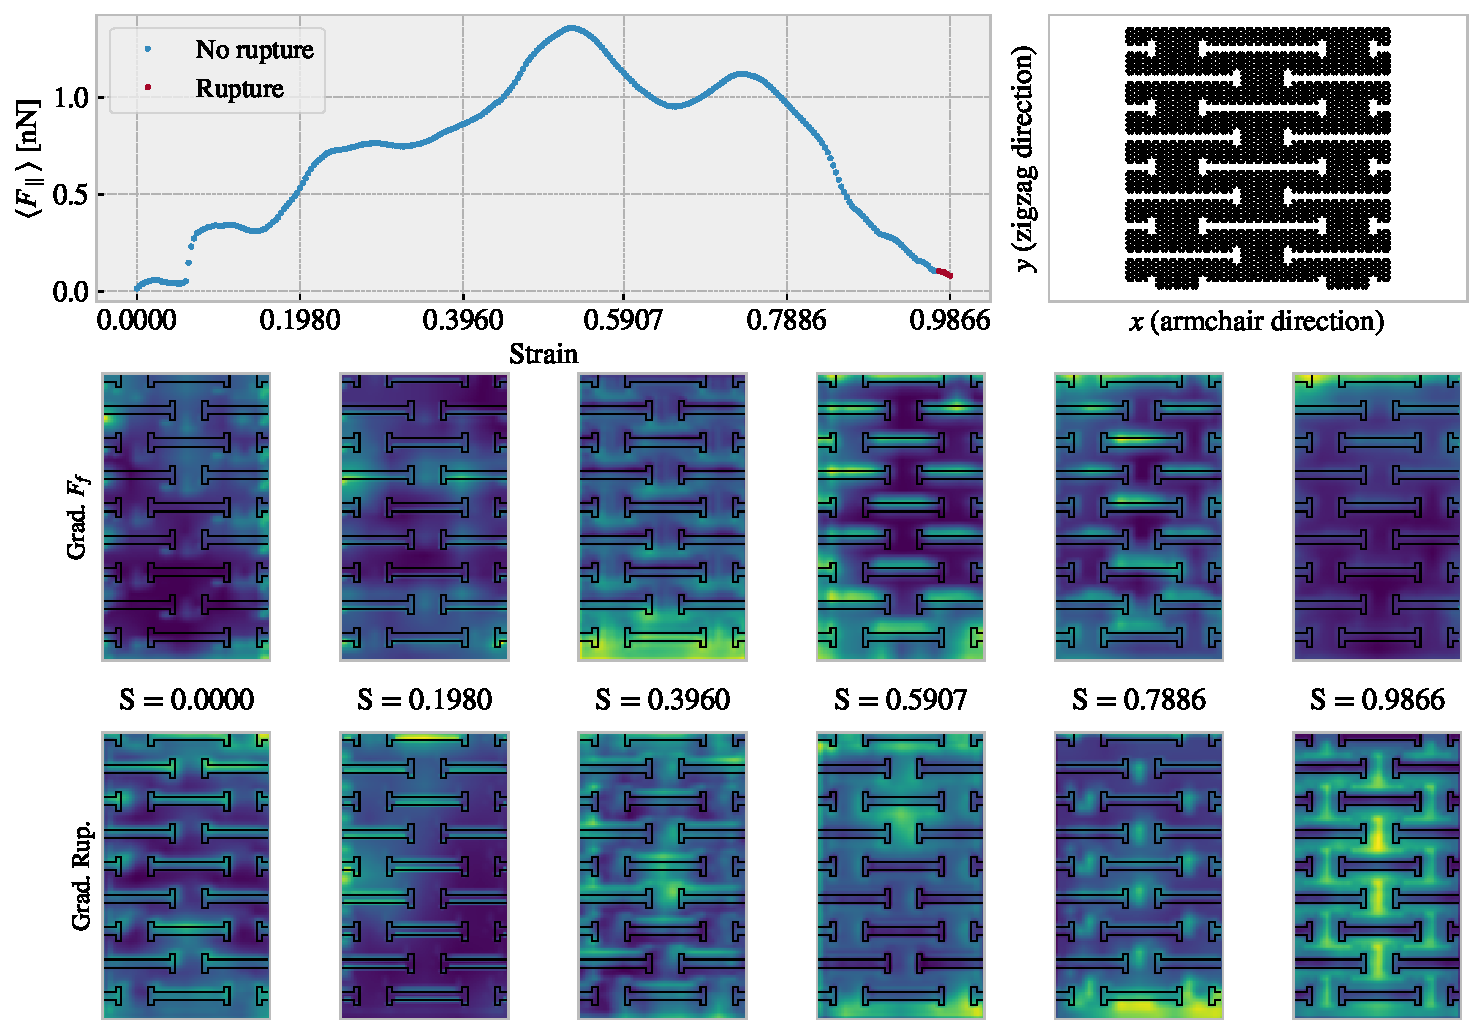
\includegraphics[width=0.8\linewidth]{figures/search/grad_cam_hon_3_3_5_3_12_0.pdf}
  \caption{Honeycomb $(3,3,5,3)$, ref = $(12,0)$}
  \label{fig:GC_hon_search}
\end{figure}  

\begin{figure}[H]
  \centering
  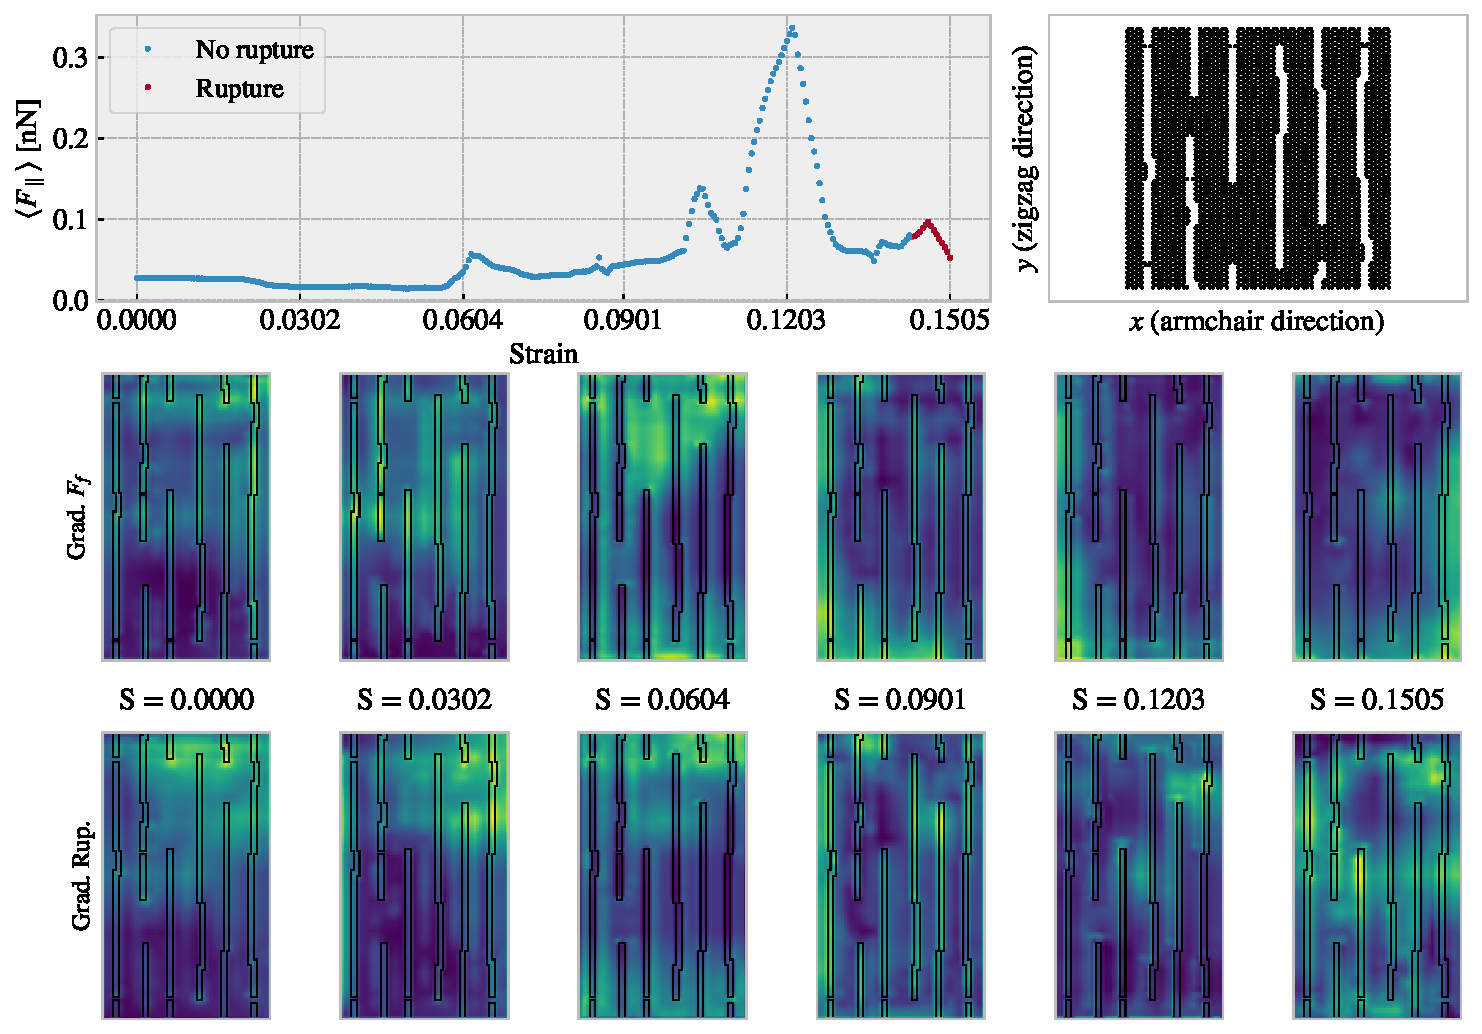
\includegraphics[width=0.8\linewidth]{figures/search/grad_cam_RW_search_max_drop0.pdf}
  \caption{RW.}
  \label{fig:GC_RW_search}
\end{figure}  




% The genetic algorithm approach could possible benefit for a consideration of 2D connections adn translation. It will force any positive patterns to be forced in their location and do not realize that making thoose repeatly will increase effect. It effectively sees every pixel like an unique gene and not really a positional property. 



